\documentclass[twoside]{book}

% Packages required by doxygen
\usepackage{calc}
\usepackage{doxygen}
\usepackage{graphicx}
\usepackage[utf8]{inputenc}
\usepackage{makeidx}
\usepackage{multicol}
\usepackage{multirow}
\usepackage{textcomp}
\usepackage[table]{xcolor}

% Font selection
\usepackage[T1]{fontenc}
\usepackage{mathptmx}
\usepackage[scaled=.90]{helvet}
\usepackage{courier}
\usepackage{amssymb}
\usepackage{sectsty}
\renewcommand{\familydefault}{\sfdefault}
\allsectionsfont{%
  \fontseries{bc}\selectfont%
  \color{darkgray}%
}
\renewcommand{\DoxyLabelFont}{%
  \fontseries{bc}\selectfont%
  \color{darkgray}%
}

% Page & text layout
\usepackage{geometry}
\geometry{%
  a4paper,%
  top=2.5cm,%
  bottom=2.5cm,%
  left=2.5cm,%
  right=2.5cm%
}
\tolerance=750
\hfuzz=15pt
\hbadness=750
\setlength{\emergencystretch}{15pt}
\setlength{\parindent}{0cm}
\setlength{\parskip}{0.2cm}
\makeatletter
\renewcommand{\paragraph}{%
  \@startsection{paragraph}{4}{0ex}{-1.0ex}{1.0ex}{%
    \normalfont\normalsize\bfseries\SS@parafont%
  }%
}
\renewcommand{\subparagraph}{%
  \@startsection{subparagraph}{5}{0ex}{-1.0ex}{1.0ex}{%
    \normalfont\normalsize\bfseries\SS@subparafont%
  }%
}
\makeatother

% Headers & footers
\usepackage{fancyhdr}
\pagestyle{fancyplain}
\fancyhead[LE]{\fancyplain{}{\bfseries\thepage}}
\fancyhead[CE]{\fancyplain{}{}}
\fancyhead[RE]{\fancyplain{}{\bfseries\leftmark}}
\fancyhead[LO]{\fancyplain{}{\bfseries\rightmark}}
\fancyhead[CO]{\fancyplain{}{}}
\fancyhead[RO]{\fancyplain{}{\bfseries\thepage}}
\fancyfoot[LE]{\fancyplain{}{}}
\fancyfoot[CE]{\fancyplain{}{}}
\fancyfoot[RE]{\fancyplain{}{\bfseries\scriptsize Generated on Tue Feb 25 2020 22\-:33\-:53 for Pong Game by Doxygen }}
\fancyfoot[LO]{\fancyplain{}{\bfseries\scriptsize Generated on Tue Feb 25 2020 22\-:33\-:53 for Pong Game by Doxygen }}
\fancyfoot[CO]{\fancyplain{}{}}
\fancyfoot[RO]{\fancyplain{}{}}
\renewcommand{\footrulewidth}{0.4pt}
\renewcommand{\chaptermark}[1]{%
  \markboth{#1}{}%
}
\renewcommand{\sectionmark}[1]{%
  \markright{\thesection\ #1}%
}

% Indices & bibliography
\usepackage{natbib}
\usepackage[titles]{tocloft}
\setcounter{tocdepth}{3}
\setcounter{secnumdepth}{5}
\makeindex

% Hyperlinks (required, but should be loaded last)
\usepackage{ifpdf}
\ifpdf
  \usepackage[pdftex,pagebackref=true]{hyperref}
\else
  \usepackage[ps2pdf,pagebackref=true]{hyperref}
\fi
\hypersetup{%
  colorlinks=true,%
  linkcolor=blue,%
  citecolor=blue,%
  unicode%
}

% Custom commands
\newcommand{\clearemptydoublepage}{%
  \newpage{\pagestyle{empty}\cleardoublepage}%
}


%===== C O N T E N T S =====

\begin{document}

% Titlepage & ToC
\hypersetup{pageanchor=false}
\pagenumbering{roman}
\begin{titlepage}
\vspace*{7cm}
\begin{center}%
{\Large Pong Game }\\
\vspace*{1cm}
{\large Generated by Doxygen 1.8.6}\\
\vspace*{0.5cm}
{\small Tue Feb 25 2020 22:33:53}\\
\end{center}
\end{titlepage}
\clearemptydoublepage
\tableofcontents
\clearemptydoublepage
\pagenumbering{arabic}
\hypersetup{pageanchor=true}

%--- Begin generated contents ---
\chapter{Pong Game}
\label{md__r_e_a_d_m_e}
\hypertarget{md__r_e_a_d_m_e}{}
This is an implementation of the classical Pong game.

\subsection*{prerequisites}


\begin{DoxyItemize}
\item Visual Studio (Available online for mac and windows)
\item Mono\-Game
\end{DoxyItemize}

\subsection*{Running}

This project can be run by using Visual Studio. Once you have the project open on visual studio, press the start button, which will compile and run the game.

\subsection*{Output}

The output should look match the following\-:



\subsection*{Playing}

This is a two player game. The left player can use the {\ttfamily W} and {\ttfamily S} keys to move up and down. The right player can use the arrow keys to move up and down. Users can reset the game by clicking {\ttfamily R} key. They can also quit the game by clicking {\ttfamily Q} or {\ttfamily E\-S\-C} key.

\subsection*{Author(s)}


\begin{DoxyItemize}
\item Abel Weldaregay (\href{mailto:abelweldaregay@gmail.com}{\tt abelweldaregay@gmail.\-com}) 
\end{DoxyItemize}
\chapter{Namespace Index}
\section{Namespace List}
Here is a list of all namespaces with brief descriptions\-:\begin{DoxyCompactList}
\item\contentsline{section}{\hyperlink{namespace_ping___pong}{Ping\-\_\-\-Pong} }{\pageref{namespace_ping___pong}}{}
\end{DoxyCompactList}

\chapter{Hierarchical Index}
\section{Class Hierarchy}
This inheritance list is sorted roughly, but not completely, alphabetically\-:\begin{DoxyCompactList}
\item Game\begin{DoxyCompactList}
\item \contentsline{section}{Ping\-\_\-\-Pong.\-Game1}{\pageref{class_ping___pong_1_1_game1}}{}
\end{DoxyCompactList}
\item \contentsline{section}{Ping\-\_\-\-Pong.\-Game\-Object}{\pageref{class_ping___pong_1_1_game_object}}{}
\begin{DoxyCompactList}
\item \contentsline{section}{Ping\-\_\-\-Pong.\-Ball}{\pageref{class_ping___pong_1_1_ball}}{}
\item \contentsline{section}{Ping\-\_\-\-Pong.\-Paddle}{\pageref{class_ping___pong_1_1_paddle}}{}
\end{DoxyCompactList}
\item \contentsline{section}{Ping\-\_\-\-Pong.\-Program}{\pageref{class_ping___pong_1_1_program}}{}
\end{DoxyCompactList}

\chapter{Data Structure Index}
\section{Data Structures}
Here are the data structures with brief descriptions\-:\begin{DoxyCompactList}
\item\contentsline{section}{\hyperlink{class_ping___pong_1_1_ball}{Ping\-\_\-\-Pong.\-Ball} }{\pageref{class_ping___pong_1_1_ball}}{}
\item\contentsline{section}{\hyperlink{class_ping___pong_1_1_game1}{Ping\-\_\-\-Pong.\-Game1} \\*This is the main type for your game }{\pageref{class_ping___pong_1_1_game1}}{}
\item\contentsline{section}{\hyperlink{class_ping___pong_1_1_game_object}{Ping\-\_\-\-Pong.\-Game\-Object} }{\pageref{class_ping___pong_1_1_game_object}}{}
\item\contentsline{section}{\hyperlink{class_ping___pong_1_1_paddle}{Ping\-\_\-\-Pong.\-Paddle} }{\pageref{class_ping___pong_1_1_paddle}}{}
\item\contentsline{section}{\hyperlink{class_ping___pong_1_1_program}{Ping\-\_\-\-Pong.\-Program} }{\pageref{class_ping___pong_1_1_program}}{}
\end{DoxyCompactList}

\chapter{File Index}
\section{File List}
Here is a list of all files with brief descriptions\-:\begin{DoxyCompactList}
\item\contentsline{section}{Pong Base/\hyperlink{_ball_8cs}{Ball.\-cs} }{\pageref{_ball_8cs}}{}
\item\contentsline{section}{Pong Base/\hyperlink{_game1_8cs}{Game1.\-cs} }{\pageref{_game1_8cs}}{}
\item\contentsline{section}{Pong Base/\hyperlink{_game_object_8cs}{Game\-Object.\-cs} }{\pageref{_game_object_8cs}}{}
\item\contentsline{section}{Pong Base/\hyperlink{_paddle_8cs}{Paddle.\-cs} }{\pageref{_paddle_8cs}}{}
\item\contentsline{section}{Pong Base/\hyperlink{_program_8cs}{Program.\-cs} }{\pageref{_program_8cs}}{}
\item\contentsline{section}{Pong Base/obj/x86/\-Debug/\hyperlink{_debug_2_temporary_generated_file__036_c0_b5_b-1481-4323-8_d20-8_f5_a_d_c_b23_d92_8cs}{Temporary\-Generated\-File\-\_\-036\-C0\-B5\-B-\/1481-\/4323-\/8\-D20-\/8\-F5\-A\-D\-C\-B23\-D92.\-cs} }{\pageref{_debug_2_temporary_generated_file__036_c0_b5_b-1481-4323-8_d20-8_f5_a_d_c_b23_d92_8cs}}{}
\item\contentsline{section}{Pong Base/obj/x86/\-Debug/\hyperlink{_debug_2_temporary_generated_file__5937a670-0e60-4077-877b-f7221da3dda1_8cs}{Temporary\-Generated\-File\-\_\-5937a670-\/0e60-\/4077-\/877b-\/f7221da3dda1.\-cs} }{\pageref{_debug_2_temporary_generated_file__5937a670-0e60-4077-877b-f7221da3dda1_8cs}}{}
\item\contentsline{section}{Pong Base/obj/x86/\-Debug/\hyperlink{_debug_2_temporary_generated_file___e7_a71_f73-0_f8_d-4_b9_b-_b56_e-8_e70_b10_b_c5_d3_8cs}{Temporary\-Generated\-File\-\_\-\-E7\-A71\-F73-\/0\-F8\-D-\/4\-B9\-B-\/\-B56\-E-\/8\-E70\-B10\-B\-C5\-D3.\-cs} }{\pageref{_debug_2_temporary_generated_file___e7_a71_f73-0_f8_d-4_b9_b-_b56_e-8_e70_b10_b_c5_d3_8cs}}{}
\item\contentsline{section}{Pong Base/obj/x86/\-Release/\hyperlink{_release_2_temporary_generated_file__036_c0_b5_b-1481-4323-8_d20-8_f5_a_d_c_b23_d92_8cs}{Temporary\-Generated\-File\-\_\-036\-C0\-B5\-B-\/1481-\/4323-\/8\-D20-\/8\-F5\-A\-D\-C\-B23\-D92.\-cs} }{\pageref{_release_2_temporary_generated_file__036_c0_b5_b-1481-4323-8_d20-8_f5_a_d_c_b23_d92_8cs}}{}
\item\contentsline{section}{Pong Base/obj/x86/\-Release/\hyperlink{_release_2_temporary_generated_file__5937a670-0e60-4077-877b-f7221da3dda1_8cs}{Temporary\-Generated\-File\-\_\-5937a670-\/0e60-\/4077-\/877b-\/f7221da3dda1.\-cs} }{\pageref{_release_2_temporary_generated_file__5937a670-0e60-4077-877b-f7221da3dda1_8cs}}{}
\item\contentsline{section}{Pong Base/obj/x86/\-Release/\hyperlink{_release_2_temporary_generated_file___e7_a71_f73-0_f8_d-4_b9_b-_b56_e-8_e70_b10_b_c5_d3_8cs}{Temporary\-Generated\-File\-\_\-\-E7\-A71\-F73-\/0\-F8\-D-\/4\-B9\-B-\/\-B56\-E-\/8\-E70\-B10\-B\-C5\-D3.\-cs} }{\pageref{_release_2_temporary_generated_file___e7_a71_f73-0_f8_d-4_b9_b-_b56_e-8_e70_b10_b_c5_d3_8cs}}{}
\item\contentsline{section}{Pong Base/\-Properties/\hyperlink{_assembly_info_8cs}{Assembly\-Info.\-cs} }{\pageref{_assembly_info_8cs}}{}
\end{DoxyCompactList}

\chapter{Namespace Documentation}
\hypertarget{namespace_ping___pong}{\section{Package Ping\-\_\-\-Pong}
\label{namespace_ping___pong}\index{Ping\-\_\-\-Pong@{Ping\-\_\-\-Pong}}
}
\subsection*{Data Structures}
\begin{DoxyCompactItemize}
\item 
class \hyperlink{class_ping___pong_1_1_ball}{Ball}
\item 
class \hyperlink{class_ping___pong_1_1_game1}{Game1}
\begin{DoxyCompactList}\small\item\em This is the main type for your game \end{DoxyCompactList}\item 
class \hyperlink{class_ping___pong_1_1_game_object}{Game\-Object}
\item 
class \hyperlink{class_ping___pong_1_1_paddle}{Paddle}
\item 
class \hyperlink{class_ping___pong_1_1_program}{Program}
\end{DoxyCompactItemize}

\chapter{Data Structure Documentation}
\hypertarget{class_ping___pong_1_1_ball}{\section{Ping\-\_\-\-Pong.\-Ball Class Reference}
\label{class_ping___pong_1_1_ball}\index{Ping\-\_\-\-Pong.\-Ball@{Ping\-\_\-\-Pong.\-Ball}}
}


Inheritance diagram for Ping\-\_\-\-Pong.\-Ball\-:
\nopagebreak
\begin{figure}[H]
\begin{center}
\leavevmode
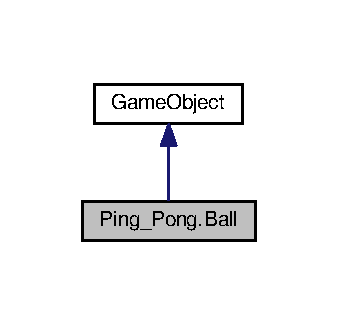
\includegraphics[width=162pt]{class_ping___pong_1_1_ball__inherit__graph}
\end{center}
\end{figure}


Collaboration diagram for Ping\-\_\-\-Pong.\-Ball\-:
\nopagebreak
\begin{figure}[H]
\begin{center}
\leavevmode
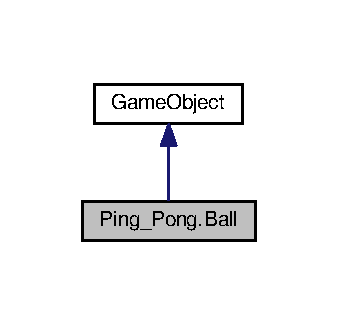
\includegraphics[width=162pt]{class_ping___pong_1_1_ball__coll__graph}
\end{center}
\end{figure}
\subsection*{Protected Attributes}
\begin{DoxyCompactItemize}
\item 
float \hyperlink{class_ping___pong_1_1_ball_abc4e830bbb71be51ce46b48cf2bd7df2}{m\-\_\-\-D\-X}
\item 
float \hyperlink{class_ping___pong_1_1_ball_a9b4627b61b519fd2ed089a277403a356}{m\-\_\-\-D\-Y}
\end{DoxyCompactItemize}
\subsection*{Properties}
\begin{DoxyCompactItemize}
\item 
float \hyperlink{class_ping___pong_1_1_ball_af3e8f435dbdb315523fd1bebb2032374}{D\-X}\hspace{0.3cm}{\ttfamily  \mbox{[}get, set\mbox{]}}
\item 
float \hyperlink{class_ping___pong_1_1_ball_a733b32b50c29c5c39e8a94654f9e3309}{D\-Y}\hspace{0.3cm}{\ttfamily  \mbox{[}get, set\mbox{]}}
\end{DoxyCompactItemize}


\subsection{Detailed Description}


Definition at line 8 of file Ball.\-cs.



\subsection{Field Documentation}
\hypertarget{class_ping___pong_1_1_ball_abc4e830bbb71be51ce46b48cf2bd7df2}{\index{Ping\-\_\-\-Pong\-::\-Ball@{Ping\-\_\-\-Pong\-::\-Ball}!m\-\_\-\-D\-X@{m\-\_\-\-D\-X}}
\index{m\-\_\-\-D\-X@{m\-\_\-\-D\-X}!Ping_Pong::Ball@{Ping\-\_\-\-Pong\-::\-Ball}}
\subsubsection[{m\-\_\-\-D\-X}]{\setlength{\rightskip}{0pt plus 5cm}float Ping\-\_\-\-Pong.\-Ball.\-m\-\_\-\-D\-X\hspace{0.3cm}{\ttfamily [protected]}}}\label{class_ping___pong_1_1_ball_abc4e830bbb71be51ce46b48cf2bd7df2}


Definition at line 10 of file Ball.\-cs.

\hypertarget{class_ping___pong_1_1_ball_a9b4627b61b519fd2ed089a277403a356}{\index{Ping\-\_\-\-Pong\-::\-Ball@{Ping\-\_\-\-Pong\-::\-Ball}!m\-\_\-\-D\-Y@{m\-\_\-\-D\-Y}}
\index{m\-\_\-\-D\-Y@{m\-\_\-\-D\-Y}!Ping_Pong::Ball@{Ping\-\_\-\-Pong\-::\-Ball}}
\subsubsection[{m\-\_\-\-D\-Y}]{\setlength{\rightskip}{0pt plus 5cm}float Ping\-\_\-\-Pong.\-Ball.\-m\-\_\-\-D\-Y\hspace{0.3cm}{\ttfamily [protected]}}}\label{class_ping___pong_1_1_ball_a9b4627b61b519fd2ed089a277403a356}


Definition at line 17 of file Ball.\-cs.



\subsection{Property Documentation}
\hypertarget{class_ping___pong_1_1_ball_af3e8f435dbdb315523fd1bebb2032374}{\index{Ping\-\_\-\-Pong\-::\-Ball@{Ping\-\_\-\-Pong\-::\-Ball}!D\-X@{D\-X}}
\index{D\-X@{D\-X}!Ping_Pong::Ball@{Ping\-\_\-\-Pong\-::\-Ball}}
\subsubsection[{D\-X}]{\setlength{\rightskip}{0pt plus 5cm}float Ping\-\_\-\-Pong.\-Ball.\-D\-X\hspace{0.3cm}{\ttfamily [get]}, {\ttfamily [set]}}}\label{class_ping___pong_1_1_ball_af3e8f435dbdb315523fd1bebb2032374}


Definition at line 12 of file Ball.\-cs.

\hypertarget{class_ping___pong_1_1_ball_a733b32b50c29c5c39e8a94654f9e3309}{\index{Ping\-\_\-\-Pong\-::\-Ball@{Ping\-\_\-\-Pong\-::\-Ball}!D\-Y@{D\-Y}}
\index{D\-Y@{D\-Y}!Ping_Pong::Ball@{Ping\-\_\-\-Pong\-::\-Ball}}
\subsubsection[{D\-Y}]{\setlength{\rightskip}{0pt plus 5cm}float Ping\-\_\-\-Pong.\-Ball.\-D\-Y\hspace{0.3cm}{\ttfamily [get]}, {\ttfamily [set]}}}\label{class_ping___pong_1_1_ball_a733b32b50c29c5c39e8a94654f9e3309}


Definition at line 19 of file Ball.\-cs.



The documentation for this class was generated from the following file\-:\begin{DoxyCompactItemize}
\item 
Pong Base/\hyperlink{_ball_8cs}{Ball.\-cs}\end{DoxyCompactItemize}

\hypertarget{class_ping___pong_1_1_game1}{\section{Ping\-\_\-\-Pong.\-Game1 Class Reference}
\label{class_ping___pong_1_1_game1}\index{Ping\-\_\-\-Pong.\-Game1@{Ping\-\_\-\-Pong.\-Game1}}
}


This is the main type for your game  




Inheritance diagram for Ping\-\_\-\-Pong.\-Game1\-:
\nopagebreak
\begin{figure}[H]
\begin{center}
\leavevmode
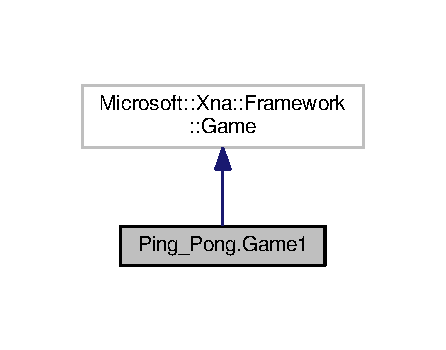
\includegraphics[width=214pt]{class_ping___pong_1_1_game1__inherit__graph}
\end{center}
\end{figure}


Collaboration diagram for Ping\-\_\-\-Pong.\-Game1\-:
\nopagebreak
\begin{figure}[H]
\begin{center}
\leavevmode
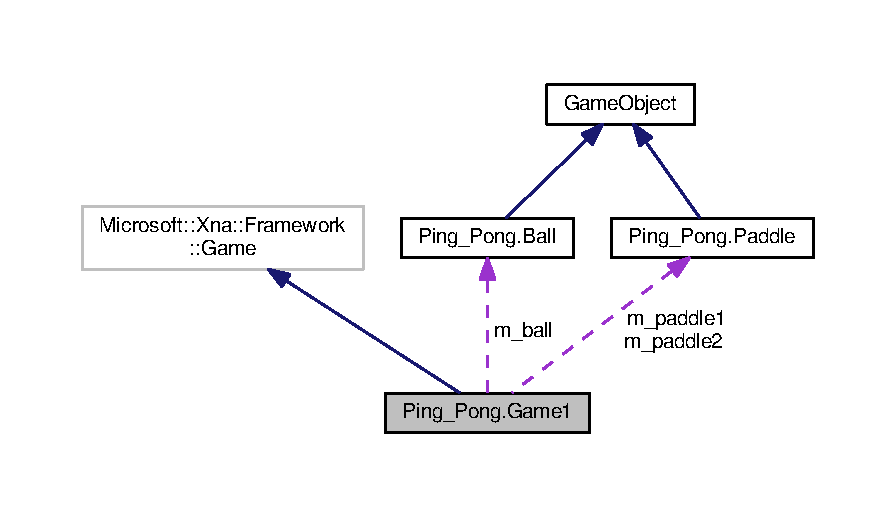
\includegraphics[width=350pt]{class_ping___pong_1_1_game1__coll__graph}
\end{center}
\end{figure}
\subsection*{Public Member Functions}
\begin{DoxyCompactItemize}
\item 
\hyperlink{class_ping___pong_1_1_game1_ab146cd91df1ef58f9a58935843ed787b}{Game1} ()
\item 
void \hyperlink{class_ping___pong_1_1_game1_a06c80c174c822247fb58b9ce3d6c18b2}{Init\-Screen} ()
\item 
void \hyperlink{class_ping___pong_1_1_game1_a18d2c9e0d2bb1f3432c54781a8c822e7}{Init\-Game\-Objects} ()
\item 
void \hyperlink{class_ping___pong_1_1_game1_a30e3122abc5d6d6555b394ef9dfea097}{Reset\-Game} ()
\item 
void \hyperlink{class_ping___pong_1_1_game1_a5e2d8c065ebbe30b5452d6e6366d21ff}{Draw\-Score} (float x, float y, int score)
\item 
void \hyperlink{class_ping___pong_1_1_game1_ad22887afd5e5fe23c2d5d218556046ee}{Render} ()
\end{DoxyCompactItemize}
\subsection*{Protected Member Functions}
\begin{DoxyCompactItemize}
\item 
override void \hyperlink{class_ping___pong_1_1_game1_ae8a0320b8583f5f671dcf98a5ca232df}{Initialize} ()
\begin{DoxyCompactList}\small\item\em Allows the game to perform any initialization it needs to before starting to run. This is where it can query for any required services and load any non-\/graphic related content. Calling base.\-Initialize will enumerate through any components and initialize them as well. \end{DoxyCompactList}\item 
override void \hyperlink{class_ping___pong_1_1_game1_a6d3747853eb20dd83968478792b1a19d}{Load\-Content} ()
\begin{DoxyCompactList}\small\item\em Load\-Content will be called once per game and is the place to load all of your content. \end{DoxyCompactList}\item 
void \hyperlink{class_ping___pong_1_1_game1_ac022f03857d45e8396e520c70eceb9c5}{Load\-Game\-Graphics} ()
\item 
override void \hyperlink{class_ping___pong_1_1_game1_a558bcf5c17e9f410d5cceb2f66e2dd67}{Unload\-Content} ()
\begin{DoxyCompactList}\small\item\em Unload\-Content will be called once per game and is the place to unload all content. \end{DoxyCompactList}\item 
override void \hyperlink{class_ping___pong_1_1_game1_adcf5d3a66fa192e3318b14188dd0c34a}{Update} (Game\-Time game\-Time)
\begin{DoxyCompactList}\small\item\em Allows the game to run logic such as updating the world, checking for collisions, gathering input, and playing audio. \end{DoxyCompactList}\item 
override void \hyperlink{class_ping___pong_1_1_game1_a4ce721b84f4194ecc1a8bf27b27f0955}{Draw} (Game\-Time game\-Time)
\begin{DoxyCompactList}\small\item\em This is called when the game should draw itself. \end{DoxyCompactList}\end{DoxyCompactItemize}
\subsection*{Private Member Functions}
\begin{DoxyCompactItemize}
\item 
void \hyperlink{class_ping___pong_1_1_game1_a61c60e00745df4154dde945cde16c7af}{Move\-Ball} ()
\item 
bool \hyperlink{class_ping___pong_1_1_game1_ad34fe9d81909ad797beb7670ebf3594d}{Collision\-Occurred} ()
\item 
void \hyperlink{class_ping___pong_1_1_game1_a545c655f415d2de1f372a6eed77e0231}{Move\-Paddles} ()
\end{DoxyCompactItemize}
\subsection*{Private Attributes}
\begin{DoxyCompactItemize}
\item 
Graphics\-Device\-Manager \hyperlink{class_ping___pong_1_1_game1_aaaff77331c3e33fc32f14a28fa530a7d}{graphics}
\item 
Sprite\-Batch \hyperlink{class_ping___pong_1_1_game1_a887077461615a43e27f62c978affad96}{sprite\-Batch}
\item 
Sprite\-Font \hyperlink{class_ping___pong_1_1_game1_adcc5e0fb3bc88b1ea3ae2c4c1a06a936}{score\-Font}
\item 
Sprite\-Font \hyperlink{class_ping___pong_1_1_game1_a1f794b8a0feab9dfdbf4c98dc86222cf}{name\-Font}
\item 
Sound\-Effect \hyperlink{class_ping___pong_1_1_game1_aaa0f5f32149b8eb6abd8c148a4e47c36}{beep}
\item 
Texture2\-D \hyperlink{class_ping___pong_1_1_game1_ae0f525562a3eb615b556f4a9a1eda3e7}{background}
\item 
Boolean \hyperlink{class_ping___pong_1_1_game1_a87f945d8a88fa041a94fe15c1446173e}{paused}
\item 
Keyboard\-State \hyperlink{class_ping___pong_1_1_game1_a13ba97510380dfbf6c00815f4d5af7ad}{old\-State}
\item 
Texture2\-D \hyperlink{class_ping___pong_1_1_game1_a2ef093c4cac7c244c30664dacecc7aa2}{pause\-Overlay}
\item 
Song \hyperlink{class_ping___pong_1_1_game1_ab6439b5c8bcfb4ba77f2a62ab4c73213}{background\-Music}
\item 
int \hyperlink{class_ping___pong_1_1_game1_a79cc64d39546f15bb7c9d169e5482444}{m\-\_\-\-Score1} = 0
\item 
int \hyperlink{class_ping___pong_1_1_game1_ad54e91077ec0e426c351258e17fb2137}{m\-\_\-\-Score2} = 0
\item 
Texture2\-D \hyperlink{class_ping___pong_1_1_game1_a7919de4eb9687284ff736962adc6d180}{m\-\_\-texture\-Numbers}
\item 
Rectangle\mbox{[}$\,$\mbox{]} \hyperlink{class_ping___pong_1_1_game1_a97f485fbb53d7daba3590705a5129e60}{m\-\_\-\-Score\-Rect} = null
\item 
\hyperlink{class_ping___pong_1_1_ball}{Ball} \hyperlink{class_ping___pong_1_1_game1_a3da763dfe56d5444101a2a3c2ea97389}{m\-\_\-ball}
\item 
Texture2\-D \hyperlink{class_ping___pong_1_1_game1_aeb0aebe72aa99d1d627260de5d1beafb}{m\-\_\-texture\-Ball}
\item 
\hyperlink{class_ping___pong_1_1_paddle}{Paddle} \hyperlink{class_ping___pong_1_1_game1_ac47e2989a6e169d42af4366f901c3d8a}{m\-\_\-paddle1}
\item 
\hyperlink{class_ping___pong_1_1_paddle}{Paddle} \hyperlink{class_ping___pong_1_1_game1_a9735bd7df2c29d6196fbba528689dfa7}{m\-\_\-paddle2}
\item 
Texture2\-D \hyperlink{class_ping___pong_1_1_game1_a2b0b61d9c93d9d11781d2d4a3c6f50d4}{m\-\_\-texture\-Paddle}
\item 
const int \hyperlink{class_ping___pong_1_1_game1_ae69f627158d80a56475c055372115b55}{S\-C\-R\-E\-E\-N\-\_\-\-W\-I\-D\-T\-H} = 640
\item 
const int \hyperlink{class_ping___pong_1_1_game1_a6128f974e5abe6615565769664daba1c}{S\-C\-R\-E\-E\-N\-\_\-\-H\-E\-I\-G\-H\-T} = 480
\item 
const float \hyperlink{class_ping___pong_1_1_game1_a4613e5c643f7d89e1d4dabb2b383bfad}{P\-A\-D\-D\-L\-E\-\_\-\-S\-T\-R\-I\-D\-E} = 10.\-0f
\end{DoxyCompactItemize}


\subsection{Detailed Description}
This is the main type for your game 



Definition at line 16 of file Game1.\-cs.



\subsection{Constructor \& Destructor Documentation}
\hypertarget{class_ping___pong_1_1_game1_ab146cd91df1ef58f9a58935843ed787b}{\index{Ping\-\_\-\-Pong\-::\-Game1@{Ping\-\_\-\-Pong\-::\-Game1}!Game1@{Game1}}
\index{Game1@{Game1}!Ping_Pong::Game1@{Ping\-\_\-\-Pong\-::\-Game1}}
\subsubsection[{Game1}]{\setlength{\rightskip}{0pt plus 5cm}Ping\-\_\-\-Pong.\-Game1.\-Game1 (
\begin{DoxyParamCaption}
{}
\end{DoxyParamCaption}
)\hspace{0.3cm}{\ttfamily [inline]}}}\label{class_ping___pong_1_1_game1_ab146cd91df1ef58f9a58935843ed787b}


Definition at line 48 of file Game1.\-cs.



\subsection{Member Function Documentation}
\hypertarget{class_ping___pong_1_1_game1_ad34fe9d81909ad797beb7670ebf3594d}{\index{Ping\-\_\-\-Pong\-::\-Game1@{Ping\-\_\-\-Pong\-::\-Game1}!Collision\-Occurred@{Collision\-Occurred}}
\index{Collision\-Occurred@{Collision\-Occurred}!Ping_Pong::Game1@{Ping\-\_\-\-Pong\-::\-Game1}}
\subsubsection[{Collision\-Occurred}]{\setlength{\rightskip}{0pt plus 5cm}bool Ping\-\_\-\-Pong.\-Game1.\-Collision\-Occurred (
\begin{DoxyParamCaption}
{}
\end{DoxyParamCaption}
)\hspace{0.3cm}{\ttfamily [inline]}, {\ttfamily [private]}}}\label{class_ping___pong_1_1_game1_ad34fe9d81909ad797beb7670ebf3594d}


Definition at line 321 of file Game1.\-cs.



Here is the caller graph for this function\-:
\nopagebreak
\begin{figure}[H]
\begin{center}
\leavevmode
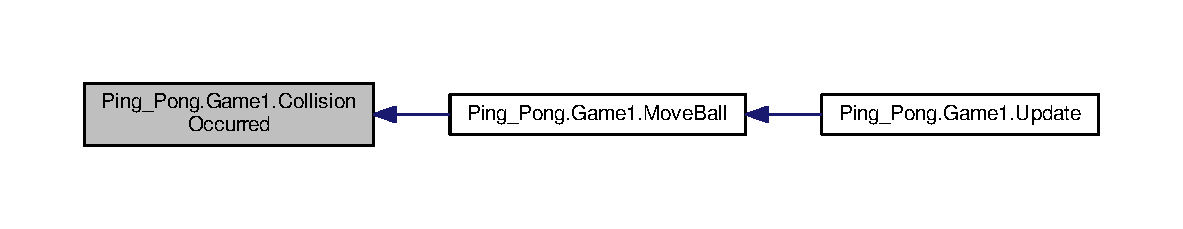
\includegraphics[width=350pt]{class_ping___pong_1_1_game1_ad34fe9d81909ad797beb7670ebf3594d_icgraph}
\end{center}
\end{figure}


\hypertarget{class_ping___pong_1_1_game1_a4ce721b84f4194ecc1a8bf27b27f0955}{\index{Ping\-\_\-\-Pong\-::\-Game1@{Ping\-\_\-\-Pong\-::\-Game1}!Draw@{Draw}}
\index{Draw@{Draw}!Ping_Pong::Game1@{Ping\-\_\-\-Pong\-::\-Game1}}
\subsubsection[{Draw}]{\setlength{\rightskip}{0pt plus 5cm}override void Ping\-\_\-\-Pong.\-Game1.\-Draw (
\begin{DoxyParamCaption}
\item[{Game\-Time}]{game\-Time}
\end{DoxyParamCaption}
)\hspace{0.3cm}{\ttfamily [inline]}, {\ttfamily [protected]}}}\label{class_ping___pong_1_1_game1_a4ce721b84f4194ecc1a8bf27b27f0955}


This is called when the game should draw itself. 


\begin{DoxyParams}{Parameters}
{\em game\-Time} & Provides a snapshot of timing values.\\
\hline
\end{DoxyParams}


Definition at line 430 of file Game1.\-cs.



Here is the call graph for this function\-:
\nopagebreak
\begin{figure}[H]
\begin{center}
\leavevmode
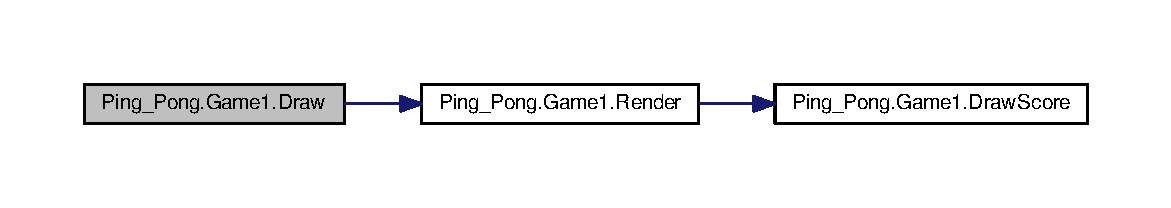
\includegraphics[width=350pt]{class_ping___pong_1_1_game1_a4ce721b84f4194ecc1a8bf27b27f0955_cgraph}
\end{center}
\end{figure}


\hypertarget{class_ping___pong_1_1_game1_a5e2d8c065ebbe30b5452d6e6366d21ff}{\index{Ping\-\_\-\-Pong\-::\-Game1@{Ping\-\_\-\-Pong\-::\-Game1}!Draw\-Score@{Draw\-Score}}
\index{Draw\-Score@{Draw\-Score}!Ping_Pong::Game1@{Ping\-\_\-\-Pong\-::\-Game1}}
\subsubsection[{Draw\-Score}]{\setlength{\rightskip}{0pt plus 5cm}void Ping\-\_\-\-Pong.\-Game1.\-Draw\-Score (
\begin{DoxyParamCaption}
\item[{float}]{x, }
\item[{float}]{y, }
\item[{int}]{score}
\end{DoxyParamCaption}
)\hspace{0.3cm}{\ttfamily [inline]}}}\label{class_ping___pong_1_1_game1_a5e2d8c065ebbe30b5452d6e6366d21ff}


Definition at line 445 of file Game1.\-cs.



Here is the caller graph for this function\-:
\nopagebreak
\begin{figure}[H]
\begin{center}
\leavevmode
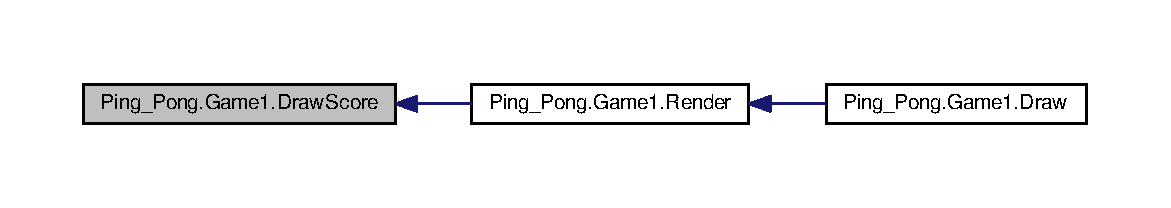
\includegraphics[width=350pt]{class_ping___pong_1_1_game1_a5e2d8c065ebbe30b5452d6e6366d21ff_icgraph}
\end{center}
\end{figure}


\hypertarget{class_ping___pong_1_1_game1_a18d2c9e0d2bb1f3432c54781a8c822e7}{\index{Ping\-\_\-\-Pong\-::\-Game1@{Ping\-\_\-\-Pong\-::\-Game1}!Init\-Game\-Objects@{Init\-Game\-Objects}}
\index{Init\-Game\-Objects@{Init\-Game\-Objects}!Ping_Pong::Game1@{Ping\-\_\-\-Pong\-::\-Game1}}
\subsubsection[{Init\-Game\-Objects}]{\setlength{\rightskip}{0pt plus 5cm}void Ping\-\_\-\-Pong.\-Game1.\-Init\-Game\-Objects (
\begin{DoxyParamCaption}
{}
\end{DoxyParamCaption}
)\hspace{0.3cm}{\ttfamily [inline]}}}\label{class_ping___pong_1_1_game1_a18d2c9e0d2bb1f3432c54781a8c822e7}


Definition at line 84 of file Game1.\-cs.



Here is the call graph for this function\-:
\nopagebreak
\begin{figure}[H]
\begin{center}
\leavevmode
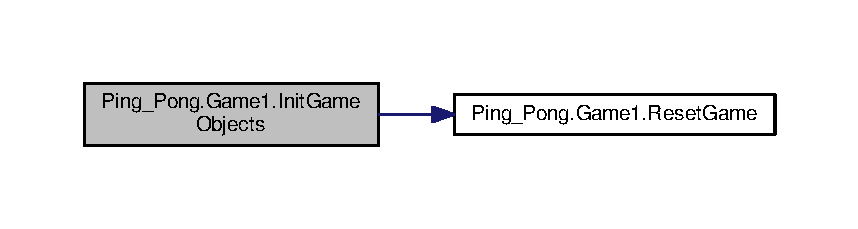
\includegraphics[width=350pt]{class_ping___pong_1_1_game1_a18d2c9e0d2bb1f3432c54781a8c822e7_cgraph}
\end{center}
\end{figure}




Here is the caller graph for this function\-:
\nopagebreak
\begin{figure}[H]
\begin{center}
\leavevmode
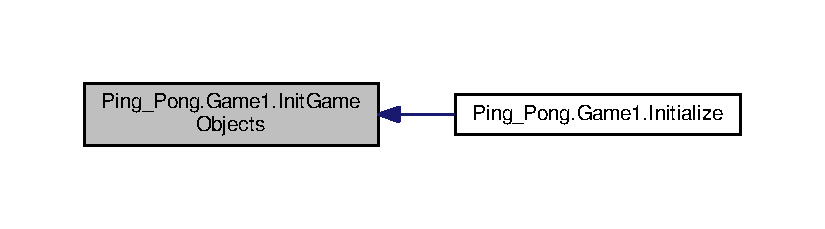
\includegraphics[width=350pt]{class_ping___pong_1_1_game1_a18d2c9e0d2bb1f3432c54781a8c822e7_icgraph}
\end{center}
\end{figure}


\hypertarget{class_ping___pong_1_1_game1_ae8a0320b8583f5f671dcf98a5ca232df}{\index{Ping\-\_\-\-Pong\-::\-Game1@{Ping\-\_\-\-Pong\-::\-Game1}!Initialize@{Initialize}}
\index{Initialize@{Initialize}!Ping_Pong::Game1@{Ping\-\_\-\-Pong\-::\-Game1}}
\subsubsection[{Initialize}]{\setlength{\rightskip}{0pt plus 5cm}override void Ping\-\_\-\-Pong.\-Game1.\-Initialize (
\begin{DoxyParamCaption}
{}
\end{DoxyParamCaption}
)\hspace{0.3cm}{\ttfamily [inline]}, {\ttfamily [protected]}}}\label{class_ping___pong_1_1_game1_ae8a0320b8583f5f671dcf98a5ca232df}


Allows the game to perform any initialization it needs to before starting to run. This is where it can query for any required services and load any non-\/graphic related content. Calling base.\-Initialize will enumerate through any components and initialize them as well. 



Definition at line 60 of file Game1.\-cs.



Here is the call graph for this function\-:
\nopagebreak
\begin{figure}[H]
\begin{center}
\leavevmode
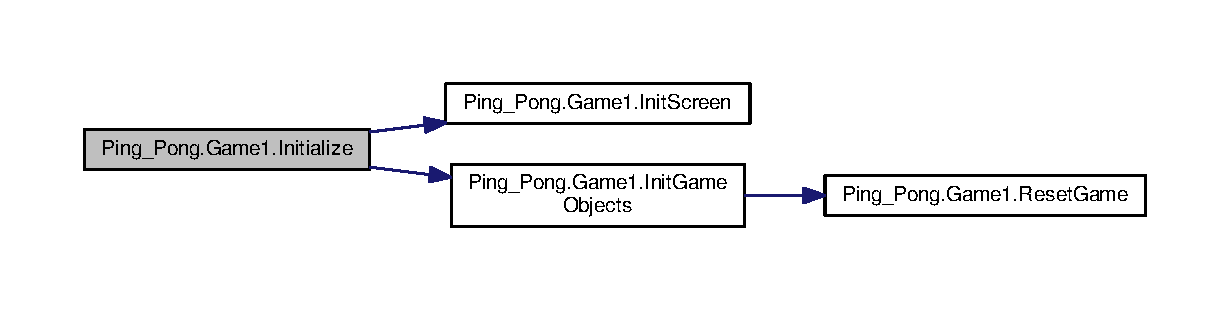
\includegraphics[width=350pt]{class_ping___pong_1_1_game1_ae8a0320b8583f5f671dcf98a5ca232df_cgraph}
\end{center}
\end{figure}


\hypertarget{class_ping___pong_1_1_game1_a06c80c174c822247fb58b9ce3d6c18b2}{\index{Ping\-\_\-\-Pong\-::\-Game1@{Ping\-\_\-\-Pong\-::\-Game1}!Init\-Screen@{Init\-Screen}}
\index{Init\-Screen@{Init\-Screen}!Ping_Pong::Game1@{Ping\-\_\-\-Pong\-::\-Game1}}
\subsubsection[{Init\-Screen}]{\setlength{\rightskip}{0pt plus 5cm}void Ping\-\_\-\-Pong.\-Game1.\-Init\-Screen (
\begin{DoxyParamCaption}
{}
\end{DoxyParamCaption}
)\hspace{0.3cm}{\ttfamily [inline]}}}\label{class_ping___pong_1_1_game1_a06c80c174c822247fb58b9ce3d6c18b2}


Definition at line 74 of file Game1.\-cs.



Here is the caller graph for this function\-:
\nopagebreak
\begin{figure}[H]
\begin{center}
\leavevmode
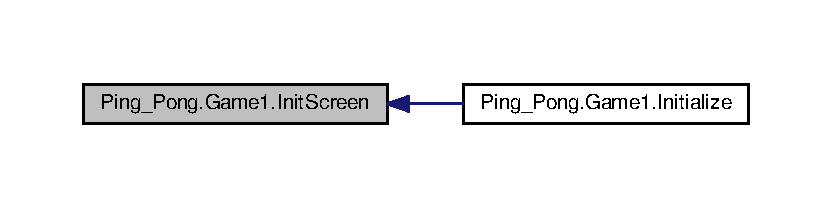
\includegraphics[width=350pt]{class_ping___pong_1_1_game1_a06c80c174c822247fb58b9ce3d6c18b2_icgraph}
\end{center}
\end{figure}


\hypertarget{class_ping___pong_1_1_game1_a6d3747853eb20dd83968478792b1a19d}{\index{Ping\-\_\-\-Pong\-::\-Game1@{Ping\-\_\-\-Pong\-::\-Game1}!Load\-Content@{Load\-Content}}
\index{Load\-Content@{Load\-Content}!Ping_Pong::Game1@{Ping\-\_\-\-Pong\-::\-Game1}}
\subsubsection[{Load\-Content}]{\setlength{\rightskip}{0pt plus 5cm}override void Ping\-\_\-\-Pong.\-Game1.\-Load\-Content (
\begin{DoxyParamCaption}
{}
\end{DoxyParamCaption}
)\hspace{0.3cm}{\ttfamily [inline]}, {\ttfamily [protected]}}}\label{class_ping___pong_1_1_game1_a6d3747853eb20dd83968478792b1a19d}


Load\-Content will be called once per game and is the place to load all of your content. 



Definition at line 160 of file Game1.\-cs.



Here is the call graph for this function\-:
\nopagebreak
\begin{figure}[H]
\begin{center}
\leavevmode
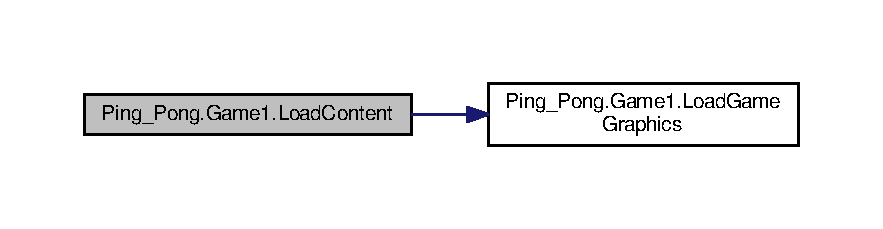
\includegraphics[width=350pt]{class_ping___pong_1_1_game1_a6d3747853eb20dd83968478792b1a19d_cgraph}
\end{center}
\end{figure}


\hypertarget{class_ping___pong_1_1_game1_ac022f03857d45e8396e520c70eceb9c5}{\index{Ping\-\_\-\-Pong\-::\-Game1@{Ping\-\_\-\-Pong\-::\-Game1}!Load\-Game\-Graphics@{Load\-Game\-Graphics}}
\index{Load\-Game\-Graphics@{Load\-Game\-Graphics}!Ping_Pong::Game1@{Ping\-\_\-\-Pong\-::\-Game1}}
\subsubsection[{Load\-Game\-Graphics}]{\setlength{\rightskip}{0pt plus 5cm}void Ping\-\_\-\-Pong.\-Game1.\-Load\-Game\-Graphics (
\begin{DoxyParamCaption}
{}
\end{DoxyParamCaption}
)\hspace{0.3cm}{\ttfamily [inline]}, {\ttfamily [protected]}}}\label{class_ping___pong_1_1_game1_ac022f03857d45e8396e520c70eceb9c5}


Definition at line 173 of file Game1.\-cs.



Here is the caller graph for this function\-:
\nopagebreak
\begin{figure}[H]
\begin{center}
\leavevmode
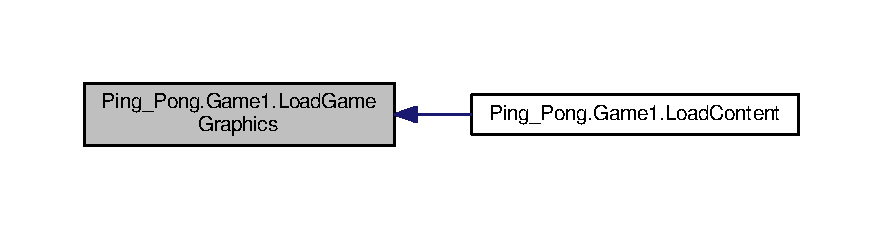
\includegraphics[width=350pt]{class_ping___pong_1_1_game1_ac022f03857d45e8396e520c70eceb9c5_icgraph}
\end{center}
\end{figure}


\hypertarget{class_ping___pong_1_1_game1_a61c60e00745df4154dde945cde16c7af}{\index{Ping\-\_\-\-Pong\-::\-Game1@{Ping\-\_\-\-Pong\-::\-Game1}!Move\-Ball@{Move\-Ball}}
\index{Move\-Ball@{Move\-Ball}!Ping_Pong::Game1@{Ping\-\_\-\-Pong\-::\-Game1}}
\subsubsection[{Move\-Ball}]{\setlength{\rightskip}{0pt plus 5cm}void Ping\-\_\-\-Pong.\-Game1.\-Move\-Ball (
\begin{DoxyParamCaption}
{}
\end{DoxyParamCaption}
)\hspace{0.3cm}{\ttfamily [inline]}, {\ttfamily [private]}}}\label{class_ping___pong_1_1_game1_a61c60e00745df4154dde945cde16c7af}


Definition at line 260 of file Game1.\-cs.



Here is the call graph for this function\-:
\nopagebreak
\begin{figure}[H]
\begin{center}
\leavevmode
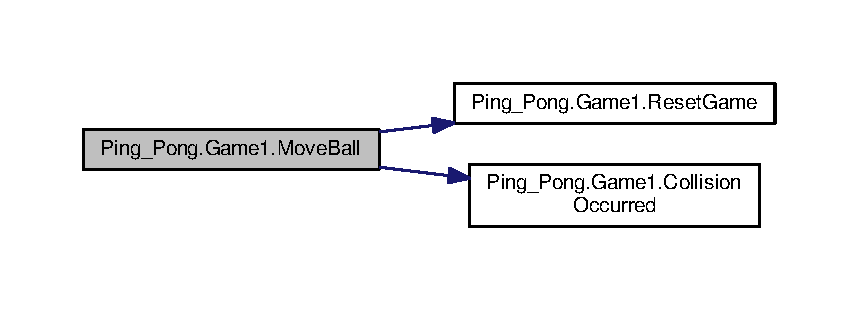
\includegraphics[width=350pt]{class_ping___pong_1_1_game1_a61c60e00745df4154dde945cde16c7af_cgraph}
\end{center}
\end{figure}




Here is the caller graph for this function\-:
\nopagebreak
\begin{figure}[H]
\begin{center}
\leavevmode
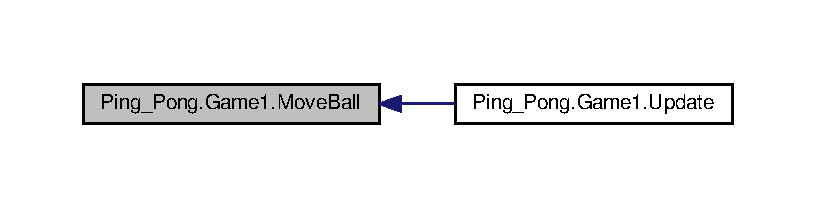
\includegraphics[width=350pt]{class_ping___pong_1_1_game1_a61c60e00745df4154dde945cde16c7af_icgraph}
\end{center}
\end{figure}


\hypertarget{class_ping___pong_1_1_game1_a545c655f415d2de1f372a6eed77e0231}{\index{Ping\-\_\-\-Pong\-::\-Game1@{Ping\-\_\-\-Pong\-::\-Game1}!Move\-Paddles@{Move\-Paddles}}
\index{Move\-Paddles@{Move\-Paddles}!Ping_Pong::Game1@{Ping\-\_\-\-Pong\-::\-Game1}}
\subsubsection[{Move\-Paddles}]{\setlength{\rightskip}{0pt plus 5cm}void Ping\-\_\-\-Pong.\-Game1.\-Move\-Paddles (
\begin{DoxyParamCaption}
{}
\end{DoxyParamCaption}
)\hspace{0.3cm}{\ttfamily [inline]}, {\ttfamily [private]}}}\label{class_ping___pong_1_1_game1_a545c655f415d2de1f372a6eed77e0231}


Definition at line 356 of file Game1.\-cs.



Here is the caller graph for this function\-:
\nopagebreak
\begin{figure}[H]
\begin{center}
\leavevmode
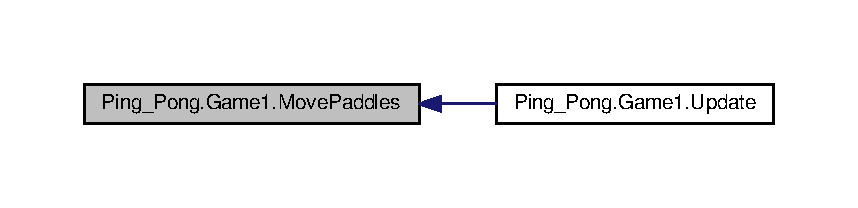
\includegraphics[width=350pt]{class_ping___pong_1_1_game1_a545c655f415d2de1f372a6eed77e0231_icgraph}
\end{center}
\end{figure}


\hypertarget{class_ping___pong_1_1_game1_ad22887afd5e5fe23c2d5d218556046ee}{\index{Ping\-\_\-\-Pong\-::\-Game1@{Ping\-\_\-\-Pong\-::\-Game1}!Render@{Render}}
\index{Render@{Render}!Ping_Pong::Game1@{Ping\-\_\-\-Pong\-::\-Game1}}
\subsubsection[{Render}]{\setlength{\rightskip}{0pt plus 5cm}void Ping\-\_\-\-Pong.\-Game1.\-Render (
\begin{DoxyParamCaption}
{}
\end{DoxyParamCaption}
)\hspace{0.3cm}{\ttfamily [inline]}}}\label{class_ping___pong_1_1_game1_ad22887afd5e5fe23c2d5d218556046ee}


Definition at line 456 of file Game1.\-cs.



Here is the call graph for this function\-:
\nopagebreak
\begin{figure}[H]
\begin{center}
\leavevmode
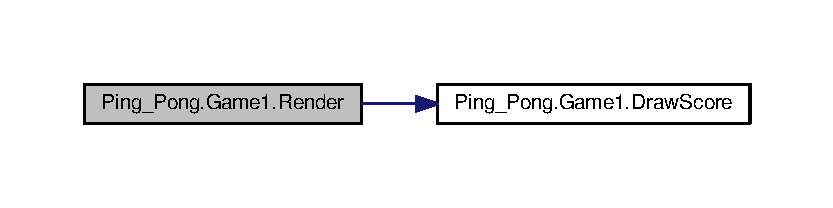
\includegraphics[width=350pt]{class_ping___pong_1_1_game1_ad22887afd5e5fe23c2d5d218556046ee_cgraph}
\end{center}
\end{figure}




Here is the caller graph for this function\-:
\nopagebreak
\begin{figure}[H]
\begin{center}
\leavevmode
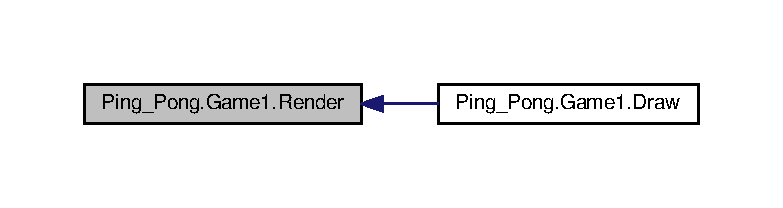
\includegraphics[width=350pt]{class_ping___pong_1_1_game1_ad22887afd5e5fe23c2d5d218556046ee_icgraph}
\end{center}
\end{figure}


\hypertarget{class_ping___pong_1_1_game1_a30e3122abc5d6d6555b394ef9dfea097}{\index{Ping\-\_\-\-Pong\-::\-Game1@{Ping\-\_\-\-Pong\-::\-Game1}!Reset\-Game@{Reset\-Game}}
\index{Reset\-Game@{Reset\-Game}!Ping_Pong::Game1@{Ping\-\_\-\-Pong\-::\-Game1}}
\subsubsection[{Reset\-Game}]{\setlength{\rightskip}{0pt plus 5cm}void Ping\-\_\-\-Pong.\-Game1.\-Reset\-Game (
\begin{DoxyParamCaption}
{}
\end{DoxyParamCaption}
)\hspace{0.3cm}{\ttfamily [inline]}}}\label{class_ping___pong_1_1_game1_a30e3122abc5d6d6555b394ef9dfea097}


Definition at line 119 of file Game1.\-cs.



Here is the caller graph for this function\-:
\nopagebreak
\begin{figure}[H]
\begin{center}
\leavevmode
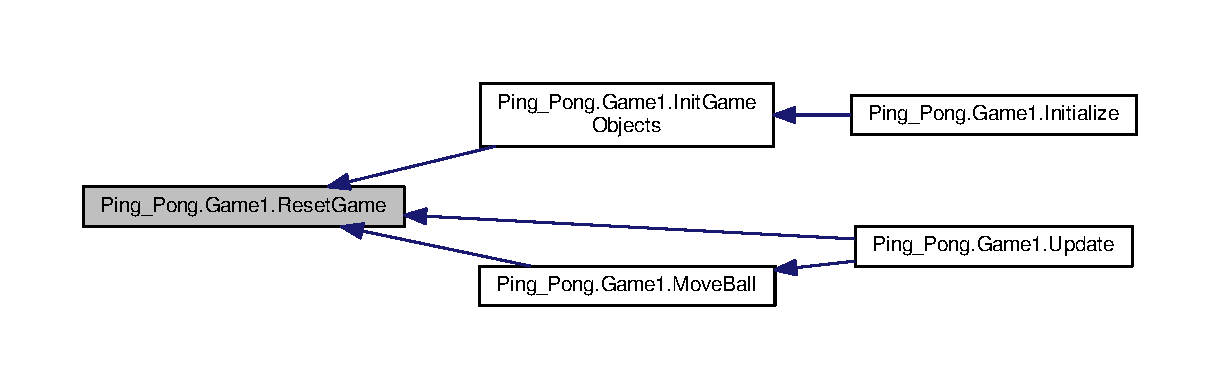
\includegraphics[width=350pt]{class_ping___pong_1_1_game1_a30e3122abc5d6d6555b394ef9dfea097_icgraph}
\end{center}
\end{figure}


\hypertarget{class_ping___pong_1_1_game1_a558bcf5c17e9f410d5cceb2f66e2dd67}{\index{Ping\-\_\-\-Pong\-::\-Game1@{Ping\-\_\-\-Pong\-::\-Game1}!Unload\-Content@{Unload\-Content}}
\index{Unload\-Content@{Unload\-Content}!Ping_Pong::Game1@{Ping\-\_\-\-Pong\-::\-Game1}}
\subsubsection[{Unload\-Content}]{\setlength{\rightskip}{0pt plus 5cm}override void Ping\-\_\-\-Pong.\-Game1.\-Unload\-Content (
\begin{DoxyParamCaption}
{}
\end{DoxyParamCaption}
)\hspace{0.3cm}{\ttfamily [inline]}, {\ttfamily [protected]}}}\label{class_ping___pong_1_1_game1_a558bcf5c17e9f410d5cceb2f66e2dd67}


Unload\-Content will be called once per game and is the place to unload all content. 



Definition at line 201 of file Game1.\-cs.

\hypertarget{class_ping___pong_1_1_game1_adcf5d3a66fa192e3318b14188dd0c34a}{\index{Ping\-\_\-\-Pong\-::\-Game1@{Ping\-\_\-\-Pong\-::\-Game1}!Update@{Update}}
\index{Update@{Update}!Ping_Pong::Game1@{Ping\-\_\-\-Pong\-::\-Game1}}
\subsubsection[{Update}]{\setlength{\rightskip}{0pt plus 5cm}override void Ping\-\_\-\-Pong.\-Game1.\-Update (
\begin{DoxyParamCaption}
\item[{Game\-Time}]{game\-Time}
\end{DoxyParamCaption}
)\hspace{0.3cm}{\ttfamily [inline]}, {\ttfamily [protected]}}}\label{class_ping___pong_1_1_game1_adcf5d3a66fa192e3318b14188dd0c34a}


Allows the game to run logic such as updating the world, checking for collisions, gathering input, and playing audio. 


\begin{DoxyParams}{Parameters}
{\em game\-Time} & Provides a snapshot of timing values.\\
\hline
\end{DoxyParams}


Definition at line 211 of file Game1.\-cs.



Here is the call graph for this function\-:
\nopagebreak
\begin{figure}[H]
\begin{center}
\leavevmode
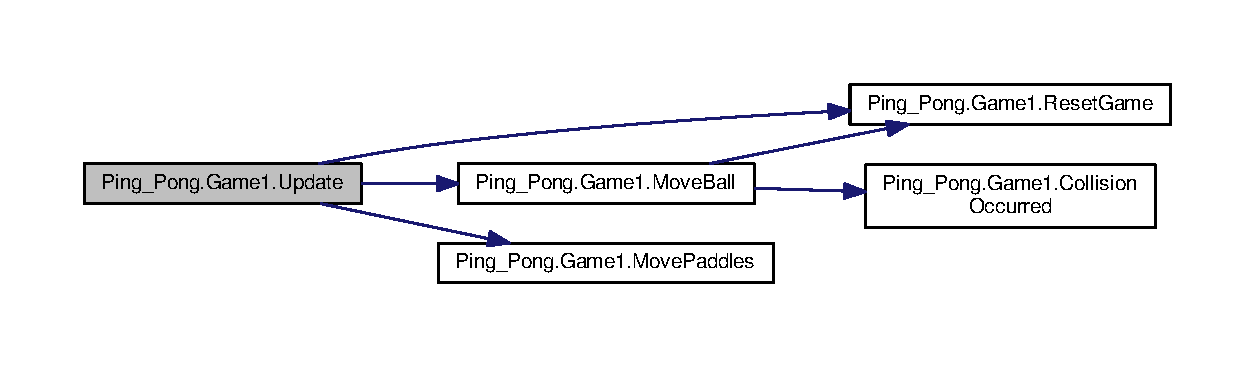
\includegraphics[width=350pt]{class_ping___pong_1_1_game1_adcf5d3a66fa192e3318b14188dd0c34a_cgraph}
\end{center}
\end{figure}




\subsection{Field Documentation}
\hypertarget{class_ping___pong_1_1_game1_ae0f525562a3eb615b556f4a9a1eda3e7}{\index{Ping\-\_\-\-Pong\-::\-Game1@{Ping\-\_\-\-Pong\-::\-Game1}!background@{background}}
\index{background@{background}!Ping_Pong::Game1@{Ping\-\_\-\-Pong\-::\-Game1}}
\subsubsection[{background}]{\setlength{\rightskip}{0pt plus 5cm}Texture2\-D Ping\-\_\-\-Pong.\-Game1.\-background\hspace{0.3cm}{\ttfamily [private]}}}\label{class_ping___pong_1_1_game1_ae0f525562a3eb615b556f4a9a1eda3e7}


Definition at line 23 of file Game1.\-cs.

\hypertarget{class_ping___pong_1_1_game1_ab6439b5c8bcfb4ba77f2a62ab4c73213}{\index{Ping\-\_\-\-Pong\-::\-Game1@{Ping\-\_\-\-Pong\-::\-Game1}!background\-Music@{background\-Music}}
\index{background\-Music@{background\-Music}!Ping_Pong::Game1@{Ping\-\_\-\-Pong\-::\-Game1}}
\subsubsection[{background\-Music}]{\setlength{\rightskip}{0pt plus 5cm}Song Ping\-\_\-\-Pong.\-Game1.\-background\-Music\hspace{0.3cm}{\ttfamily [private]}}}\label{class_ping___pong_1_1_game1_ab6439b5c8bcfb4ba77f2a62ab4c73213}


Definition at line 27 of file Game1.\-cs.

\hypertarget{class_ping___pong_1_1_game1_aaa0f5f32149b8eb6abd8c148a4e47c36}{\index{Ping\-\_\-\-Pong\-::\-Game1@{Ping\-\_\-\-Pong\-::\-Game1}!beep@{beep}}
\index{beep@{beep}!Ping_Pong::Game1@{Ping\-\_\-\-Pong\-::\-Game1}}
\subsubsection[{beep}]{\setlength{\rightskip}{0pt plus 5cm}Sound\-Effect Ping\-\_\-\-Pong.\-Game1.\-beep\hspace{0.3cm}{\ttfamily [private]}}}\label{class_ping___pong_1_1_game1_aaa0f5f32149b8eb6abd8c148a4e47c36}


Definition at line 22 of file Game1.\-cs.

\hypertarget{class_ping___pong_1_1_game1_aaaff77331c3e33fc32f14a28fa530a7d}{\index{Ping\-\_\-\-Pong\-::\-Game1@{Ping\-\_\-\-Pong\-::\-Game1}!graphics@{graphics}}
\index{graphics@{graphics}!Ping_Pong::Game1@{Ping\-\_\-\-Pong\-::\-Game1}}
\subsubsection[{graphics}]{\setlength{\rightskip}{0pt plus 5cm}Graphics\-Device\-Manager Ping\-\_\-\-Pong.\-Game1.\-graphics\hspace{0.3cm}{\ttfamily [private]}}}\label{class_ping___pong_1_1_game1_aaaff77331c3e33fc32f14a28fa530a7d}


Definition at line 18 of file Game1.\-cs.

\hypertarget{class_ping___pong_1_1_game1_a3da763dfe56d5444101a2a3c2ea97389}{\index{Ping\-\_\-\-Pong\-::\-Game1@{Ping\-\_\-\-Pong\-::\-Game1}!m\-\_\-ball@{m\-\_\-ball}}
\index{m\-\_\-ball@{m\-\_\-ball}!Ping_Pong::Game1@{Ping\-\_\-\-Pong\-::\-Game1}}
\subsubsection[{m\-\_\-ball}]{\setlength{\rightskip}{0pt plus 5cm}{\bf Ball} Ping\-\_\-\-Pong.\-Game1.\-m\-\_\-ball\hspace{0.3cm}{\ttfamily [private]}}}\label{class_ping___pong_1_1_game1_a3da763dfe56d5444101a2a3c2ea97389}


Definition at line 36 of file Game1.\-cs.

\hypertarget{class_ping___pong_1_1_game1_ac47e2989a6e169d42af4366f901c3d8a}{\index{Ping\-\_\-\-Pong\-::\-Game1@{Ping\-\_\-\-Pong\-::\-Game1}!m\-\_\-paddle1@{m\-\_\-paddle1}}
\index{m\-\_\-paddle1@{m\-\_\-paddle1}!Ping_Pong::Game1@{Ping\-\_\-\-Pong\-::\-Game1}}
\subsubsection[{m\-\_\-paddle1}]{\setlength{\rightskip}{0pt plus 5cm}{\bf Paddle} Ping\-\_\-\-Pong.\-Game1.\-m\-\_\-paddle1\hspace{0.3cm}{\ttfamily [private]}}}\label{class_ping___pong_1_1_game1_ac47e2989a6e169d42af4366f901c3d8a}


Definition at line 40 of file Game1.\-cs.

\hypertarget{class_ping___pong_1_1_game1_a9735bd7df2c29d6196fbba528689dfa7}{\index{Ping\-\_\-\-Pong\-::\-Game1@{Ping\-\_\-\-Pong\-::\-Game1}!m\-\_\-paddle2@{m\-\_\-paddle2}}
\index{m\-\_\-paddle2@{m\-\_\-paddle2}!Ping_Pong::Game1@{Ping\-\_\-\-Pong\-::\-Game1}}
\subsubsection[{m\-\_\-paddle2}]{\setlength{\rightskip}{0pt plus 5cm}{\bf Paddle} Ping\-\_\-\-Pong.\-Game1.\-m\-\_\-paddle2\hspace{0.3cm}{\ttfamily [private]}}}\label{class_ping___pong_1_1_game1_a9735bd7df2c29d6196fbba528689dfa7}


Definition at line 41 of file Game1.\-cs.

\hypertarget{class_ping___pong_1_1_game1_a79cc64d39546f15bb7c9d169e5482444}{\index{Ping\-\_\-\-Pong\-::\-Game1@{Ping\-\_\-\-Pong\-::\-Game1}!m\-\_\-\-Score1@{m\-\_\-\-Score1}}
\index{m\-\_\-\-Score1@{m\-\_\-\-Score1}!Ping_Pong::Game1@{Ping\-\_\-\-Pong\-::\-Game1}}
\subsubsection[{m\-\_\-\-Score1}]{\setlength{\rightskip}{0pt plus 5cm}int Ping\-\_\-\-Pong.\-Game1.\-m\-\_\-\-Score1 = 0\hspace{0.3cm}{\ttfamily [private]}}}\label{class_ping___pong_1_1_game1_a79cc64d39546f15bb7c9d169e5482444}


Definition at line 30 of file Game1.\-cs.

\hypertarget{class_ping___pong_1_1_game1_ad54e91077ec0e426c351258e17fb2137}{\index{Ping\-\_\-\-Pong\-::\-Game1@{Ping\-\_\-\-Pong\-::\-Game1}!m\-\_\-\-Score2@{m\-\_\-\-Score2}}
\index{m\-\_\-\-Score2@{m\-\_\-\-Score2}!Ping_Pong::Game1@{Ping\-\_\-\-Pong\-::\-Game1}}
\subsubsection[{m\-\_\-\-Score2}]{\setlength{\rightskip}{0pt plus 5cm}int Ping\-\_\-\-Pong.\-Game1.\-m\-\_\-\-Score2 = 0\hspace{0.3cm}{\ttfamily [private]}}}\label{class_ping___pong_1_1_game1_ad54e91077ec0e426c351258e17fb2137}


Definition at line 31 of file Game1.\-cs.

\hypertarget{class_ping___pong_1_1_game1_a97f485fbb53d7daba3590705a5129e60}{\index{Ping\-\_\-\-Pong\-::\-Game1@{Ping\-\_\-\-Pong\-::\-Game1}!m\-\_\-\-Score\-Rect@{m\-\_\-\-Score\-Rect}}
\index{m\-\_\-\-Score\-Rect@{m\-\_\-\-Score\-Rect}!Ping_Pong::Game1@{Ping\-\_\-\-Pong\-::\-Game1}}
\subsubsection[{m\-\_\-\-Score\-Rect}]{\setlength{\rightskip}{0pt plus 5cm}Rectangle \mbox{[}$\,$\mbox{]} Ping\-\_\-\-Pong.\-Game1.\-m\-\_\-\-Score\-Rect = null\hspace{0.3cm}{\ttfamily [private]}}}\label{class_ping___pong_1_1_game1_a97f485fbb53d7daba3590705a5129e60}


Definition at line 33 of file Game1.\-cs.

\hypertarget{class_ping___pong_1_1_game1_aeb0aebe72aa99d1d627260de5d1beafb}{\index{Ping\-\_\-\-Pong\-::\-Game1@{Ping\-\_\-\-Pong\-::\-Game1}!m\-\_\-texture\-Ball@{m\-\_\-texture\-Ball}}
\index{m\-\_\-texture\-Ball@{m\-\_\-texture\-Ball}!Ping_Pong::Game1@{Ping\-\_\-\-Pong\-::\-Game1}}
\subsubsection[{m\-\_\-texture\-Ball}]{\setlength{\rightskip}{0pt plus 5cm}Texture2\-D Ping\-\_\-\-Pong.\-Game1.\-m\-\_\-texture\-Ball\hspace{0.3cm}{\ttfamily [private]}}}\label{class_ping___pong_1_1_game1_aeb0aebe72aa99d1d627260de5d1beafb}


Definition at line 37 of file Game1.\-cs.

\hypertarget{class_ping___pong_1_1_game1_a7919de4eb9687284ff736962adc6d180}{\index{Ping\-\_\-\-Pong\-::\-Game1@{Ping\-\_\-\-Pong\-::\-Game1}!m\-\_\-texture\-Numbers@{m\-\_\-texture\-Numbers}}
\index{m\-\_\-texture\-Numbers@{m\-\_\-texture\-Numbers}!Ping_Pong::Game1@{Ping\-\_\-\-Pong\-::\-Game1}}
\subsubsection[{m\-\_\-texture\-Numbers}]{\setlength{\rightskip}{0pt plus 5cm}Texture2\-D Ping\-\_\-\-Pong.\-Game1.\-m\-\_\-texture\-Numbers\hspace{0.3cm}{\ttfamily [private]}}}\label{class_ping___pong_1_1_game1_a7919de4eb9687284ff736962adc6d180}


Definition at line 32 of file Game1.\-cs.

\hypertarget{class_ping___pong_1_1_game1_a2b0b61d9c93d9d11781d2d4a3c6f50d4}{\index{Ping\-\_\-\-Pong\-::\-Game1@{Ping\-\_\-\-Pong\-::\-Game1}!m\-\_\-texture\-Paddle@{m\-\_\-texture\-Paddle}}
\index{m\-\_\-texture\-Paddle@{m\-\_\-texture\-Paddle}!Ping_Pong::Game1@{Ping\-\_\-\-Pong\-::\-Game1}}
\subsubsection[{m\-\_\-texture\-Paddle}]{\setlength{\rightskip}{0pt plus 5cm}Texture2\-D Ping\-\_\-\-Pong.\-Game1.\-m\-\_\-texture\-Paddle\hspace{0.3cm}{\ttfamily [private]}}}\label{class_ping___pong_1_1_game1_a2b0b61d9c93d9d11781d2d4a3c6f50d4}


Definition at line 42 of file Game1.\-cs.

\hypertarget{class_ping___pong_1_1_game1_a1f794b8a0feab9dfdbf4c98dc86222cf}{\index{Ping\-\_\-\-Pong\-::\-Game1@{Ping\-\_\-\-Pong\-::\-Game1}!name\-Font@{name\-Font}}
\index{name\-Font@{name\-Font}!Ping_Pong::Game1@{Ping\-\_\-\-Pong\-::\-Game1}}
\subsubsection[{name\-Font}]{\setlength{\rightskip}{0pt plus 5cm}Sprite\-Font Ping\-\_\-\-Pong.\-Game1.\-name\-Font\hspace{0.3cm}{\ttfamily [private]}}}\label{class_ping___pong_1_1_game1_a1f794b8a0feab9dfdbf4c98dc86222cf}


Definition at line 21 of file Game1.\-cs.

\hypertarget{class_ping___pong_1_1_game1_a13ba97510380dfbf6c00815f4d5af7ad}{\index{Ping\-\_\-\-Pong\-::\-Game1@{Ping\-\_\-\-Pong\-::\-Game1}!old\-State@{old\-State}}
\index{old\-State@{old\-State}!Ping_Pong::Game1@{Ping\-\_\-\-Pong\-::\-Game1}}
\subsubsection[{old\-State}]{\setlength{\rightskip}{0pt plus 5cm}Keyboard\-State Ping\-\_\-\-Pong.\-Game1.\-old\-State\hspace{0.3cm}{\ttfamily [private]}}}\label{class_ping___pong_1_1_game1_a13ba97510380dfbf6c00815f4d5af7ad}


Definition at line 25 of file Game1.\-cs.

\hypertarget{class_ping___pong_1_1_game1_a4613e5c643f7d89e1d4dabb2b383bfad}{\index{Ping\-\_\-\-Pong\-::\-Game1@{Ping\-\_\-\-Pong\-::\-Game1}!P\-A\-D\-D\-L\-E\-\_\-\-S\-T\-R\-I\-D\-E@{P\-A\-D\-D\-L\-E\-\_\-\-S\-T\-R\-I\-D\-E}}
\index{P\-A\-D\-D\-L\-E\-\_\-\-S\-T\-R\-I\-D\-E@{P\-A\-D\-D\-L\-E\-\_\-\-S\-T\-R\-I\-D\-E}!Ping_Pong::Game1@{Ping\-\_\-\-Pong\-::\-Game1}}
\subsubsection[{P\-A\-D\-D\-L\-E\-\_\-\-S\-T\-R\-I\-D\-E}]{\setlength{\rightskip}{0pt plus 5cm}const float Ping\-\_\-\-Pong.\-Game1.\-P\-A\-D\-D\-L\-E\-\_\-\-S\-T\-R\-I\-D\-E = 10.\-0f\hspace{0.3cm}{\ttfamily [private]}}}\label{class_ping___pong_1_1_game1_a4613e5c643f7d89e1d4dabb2b383bfad}


Definition at line 353 of file Game1.\-cs.

\hypertarget{class_ping___pong_1_1_game1_a87f945d8a88fa041a94fe15c1446173e}{\index{Ping\-\_\-\-Pong\-::\-Game1@{Ping\-\_\-\-Pong\-::\-Game1}!paused@{paused}}
\index{paused@{paused}!Ping_Pong::Game1@{Ping\-\_\-\-Pong\-::\-Game1}}
\subsubsection[{paused}]{\setlength{\rightskip}{0pt plus 5cm}Boolean Ping\-\_\-\-Pong.\-Game1.\-paused\hspace{0.3cm}{\ttfamily [private]}}}\label{class_ping___pong_1_1_game1_a87f945d8a88fa041a94fe15c1446173e}


Definition at line 24 of file Game1.\-cs.

\hypertarget{class_ping___pong_1_1_game1_a2ef093c4cac7c244c30664dacecc7aa2}{\index{Ping\-\_\-\-Pong\-::\-Game1@{Ping\-\_\-\-Pong\-::\-Game1}!pause\-Overlay@{pause\-Overlay}}
\index{pause\-Overlay@{pause\-Overlay}!Ping_Pong::Game1@{Ping\-\_\-\-Pong\-::\-Game1}}
\subsubsection[{pause\-Overlay}]{\setlength{\rightskip}{0pt plus 5cm}Texture2\-D Ping\-\_\-\-Pong.\-Game1.\-pause\-Overlay\hspace{0.3cm}{\ttfamily [private]}}}\label{class_ping___pong_1_1_game1_a2ef093c4cac7c244c30664dacecc7aa2}


Definition at line 26 of file Game1.\-cs.

\hypertarget{class_ping___pong_1_1_game1_adcc5e0fb3bc88b1ea3ae2c4c1a06a936}{\index{Ping\-\_\-\-Pong\-::\-Game1@{Ping\-\_\-\-Pong\-::\-Game1}!score\-Font@{score\-Font}}
\index{score\-Font@{score\-Font}!Ping_Pong::Game1@{Ping\-\_\-\-Pong\-::\-Game1}}
\subsubsection[{score\-Font}]{\setlength{\rightskip}{0pt plus 5cm}Sprite\-Font Ping\-\_\-\-Pong.\-Game1.\-score\-Font\hspace{0.3cm}{\ttfamily [private]}}}\label{class_ping___pong_1_1_game1_adcc5e0fb3bc88b1ea3ae2c4c1a06a936}


Definition at line 20 of file Game1.\-cs.

\hypertarget{class_ping___pong_1_1_game1_a6128f974e5abe6615565769664daba1c}{\index{Ping\-\_\-\-Pong\-::\-Game1@{Ping\-\_\-\-Pong\-::\-Game1}!S\-C\-R\-E\-E\-N\-\_\-\-H\-E\-I\-G\-H\-T@{S\-C\-R\-E\-E\-N\-\_\-\-H\-E\-I\-G\-H\-T}}
\index{S\-C\-R\-E\-E\-N\-\_\-\-H\-E\-I\-G\-H\-T@{S\-C\-R\-E\-E\-N\-\_\-\-H\-E\-I\-G\-H\-T}!Ping_Pong::Game1@{Ping\-\_\-\-Pong\-::\-Game1}}
\subsubsection[{S\-C\-R\-E\-E\-N\-\_\-\-H\-E\-I\-G\-H\-T}]{\setlength{\rightskip}{0pt plus 5cm}const int Ping\-\_\-\-Pong.\-Game1.\-S\-C\-R\-E\-E\-N\-\_\-\-H\-E\-I\-G\-H\-T = 480\hspace{0.3cm}{\ttfamily [private]}}}\label{class_ping___pong_1_1_game1_a6128f974e5abe6615565769664daba1c}


Definition at line 46 of file Game1.\-cs.

\hypertarget{class_ping___pong_1_1_game1_ae69f627158d80a56475c055372115b55}{\index{Ping\-\_\-\-Pong\-::\-Game1@{Ping\-\_\-\-Pong\-::\-Game1}!S\-C\-R\-E\-E\-N\-\_\-\-W\-I\-D\-T\-H@{S\-C\-R\-E\-E\-N\-\_\-\-W\-I\-D\-T\-H}}
\index{S\-C\-R\-E\-E\-N\-\_\-\-W\-I\-D\-T\-H@{S\-C\-R\-E\-E\-N\-\_\-\-W\-I\-D\-T\-H}!Ping_Pong::Game1@{Ping\-\_\-\-Pong\-::\-Game1}}
\subsubsection[{S\-C\-R\-E\-E\-N\-\_\-\-W\-I\-D\-T\-H}]{\setlength{\rightskip}{0pt plus 5cm}const int Ping\-\_\-\-Pong.\-Game1.\-S\-C\-R\-E\-E\-N\-\_\-\-W\-I\-D\-T\-H = 640\hspace{0.3cm}{\ttfamily [private]}}}\label{class_ping___pong_1_1_game1_ae69f627158d80a56475c055372115b55}


Definition at line 45 of file Game1.\-cs.

\hypertarget{class_ping___pong_1_1_game1_a887077461615a43e27f62c978affad96}{\index{Ping\-\_\-\-Pong\-::\-Game1@{Ping\-\_\-\-Pong\-::\-Game1}!sprite\-Batch@{sprite\-Batch}}
\index{sprite\-Batch@{sprite\-Batch}!Ping_Pong::Game1@{Ping\-\_\-\-Pong\-::\-Game1}}
\subsubsection[{sprite\-Batch}]{\setlength{\rightskip}{0pt plus 5cm}Sprite\-Batch Ping\-\_\-\-Pong.\-Game1.\-sprite\-Batch\hspace{0.3cm}{\ttfamily [private]}}}\label{class_ping___pong_1_1_game1_a887077461615a43e27f62c978affad96}


Definition at line 19 of file Game1.\-cs.



The documentation for this class was generated from the following file\-:\begin{DoxyCompactItemize}
\item 
Pong Base/\hyperlink{_game1_8cs}{Game1.\-cs}\end{DoxyCompactItemize}

\hypertarget{class_ping___pong_1_1_game_object}{\section{Ping\-\_\-\-Pong.\-Game\-Object Class Reference}
\label{class_ping___pong_1_1_game_object}\index{Ping\-\_\-\-Pong.\-Game\-Object@{Ping\-\_\-\-Pong.\-Game\-Object}}
}


Inheritance diagram for Ping\-\_\-\-Pong.\-Game\-Object\-:
\nopagebreak
\begin{figure}[H]
\begin{center}
\leavevmode
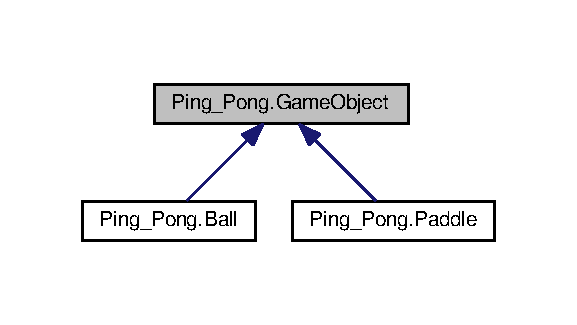
\includegraphics[width=277pt]{class_ping___pong_1_1_game_object__inherit__graph}
\end{center}
\end{figure}
\subsection*{Protected Attributes}
\begin{DoxyCompactItemize}
\item 
float \hyperlink{class_ping___pong_1_1_game_object_a292627bfcfe03c2f5a1dc403faa37690}{m\-\_\-\-X}
\item 
float \hyperlink{class_ping___pong_1_1_game_object_a29466cb57b6ac26e58052b2517083745}{m\-\_\-\-Y}
\item 
float \hyperlink{class_ping___pong_1_1_game_object_ac75ebfdec034a75ed71dbf91eface23f}{m\-\_\-\-Width}
\item 
float \hyperlink{class_ping___pong_1_1_game_object_a22de23272c1b02fb7bf7b13da7804afb}{m\-\_\-\-Height}
\item 
object \hyperlink{class_ping___pong_1_1_game_object_a5009be35d8fba10d72173a954caef57c}{m\-\_\-\-Visual} = null
\end{DoxyCompactItemize}
\subsection*{Properties}
\begin{DoxyCompactItemize}
\item 
float \hyperlink{class_ping___pong_1_1_game_object_ada20bb1f95db380d4c1af7c2030b0c1b}{X}\hspace{0.3cm}{\ttfamily  \mbox{[}get, set\mbox{]}}
\item 
float \hyperlink{class_ping___pong_1_1_game_object_adf561c4e05f7c2f4032d8302e01a3967}{Y}\hspace{0.3cm}{\ttfamily  \mbox{[}get, set\mbox{]}}
\item 
float \hyperlink{class_ping___pong_1_1_game_object_a828f5327d84be8a61d48534b2dc39e92}{Width}\hspace{0.3cm}{\ttfamily  \mbox{[}get, set\mbox{]}}
\item 
float \hyperlink{class_ping___pong_1_1_game_object_a66385f8db21929ffb9fa7f180db54f95}{Height}\hspace{0.3cm}{\ttfamily  \mbox{[}get, set\mbox{]}}
\item 
Rectangle \hyperlink{class_ping___pong_1_1_game_object_a2f69360b5ba37b1ebb3cc324244060c2}{Rect}\hspace{0.3cm}{\ttfamily  \mbox{[}get\mbox{]}}
\item 
object \hyperlink{class_ping___pong_1_1_game_object_ab7e73702e83fa5d455e191551fe86b22}{Visual}\hspace{0.3cm}{\ttfamily  \mbox{[}get, set\mbox{]}}
\end{DoxyCompactItemize}


\subsection{Detailed Description}


Definition at line 9 of file Game\-Object.\-cs.



\subsection{Field Documentation}
\hypertarget{class_ping___pong_1_1_game_object_a22de23272c1b02fb7bf7b13da7804afb}{\index{Ping\-\_\-\-Pong\-::\-Game\-Object@{Ping\-\_\-\-Pong\-::\-Game\-Object}!m\-\_\-\-Height@{m\-\_\-\-Height}}
\index{m\-\_\-\-Height@{m\-\_\-\-Height}!Ping_Pong::GameObject@{Ping\-\_\-\-Pong\-::\-Game\-Object}}
\subsubsection[{m\-\_\-\-Height}]{\setlength{\rightskip}{0pt plus 5cm}float Ping\-\_\-\-Pong.\-Game\-Object.\-m\-\_\-\-Height\hspace{0.3cm}{\ttfamily [protected]}}}\label{class_ping___pong_1_1_game_object_a22de23272c1b02fb7bf7b13da7804afb}


Definition at line 32 of file Game\-Object.\-cs.

\hypertarget{class_ping___pong_1_1_game_object_a5009be35d8fba10d72173a954caef57c}{\index{Ping\-\_\-\-Pong\-::\-Game\-Object@{Ping\-\_\-\-Pong\-::\-Game\-Object}!m\-\_\-\-Visual@{m\-\_\-\-Visual}}
\index{m\-\_\-\-Visual@{m\-\_\-\-Visual}!Ping_Pong::GameObject@{Ping\-\_\-\-Pong\-::\-Game\-Object}}
\subsubsection[{m\-\_\-\-Visual}]{\setlength{\rightskip}{0pt plus 5cm}object Ping\-\_\-\-Pong.\-Game\-Object.\-m\-\_\-\-Visual = null\hspace{0.3cm}{\ttfamily [protected]}}}\label{class_ping___pong_1_1_game_object_a5009be35d8fba10d72173a954caef57c}


Definition at line 44 of file Game\-Object.\-cs.

\hypertarget{class_ping___pong_1_1_game_object_ac75ebfdec034a75ed71dbf91eface23f}{\index{Ping\-\_\-\-Pong\-::\-Game\-Object@{Ping\-\_\-\-Pong\-::\-Game\-Object}!m\-\_\-\-Width@{m\-\_\-\-Width}}
\index{m\-\_\-\-Width@{m\-\_\-\-Width}!Ping_Pong::GameObject@{Ping\-\_\-\-Pong\-::\-Game\-Object}}
\subsubsection[{m\-\_\-\-Width}]{\setlength{\rightskip}{0pt plus 5cm}float Ping\-\_\-\-Pong.\-Game\-Object.\-m\-\_\-\-Width\hspace{0.3cm}{\ttfamily [protected]}}}\label{class_ping___pong_1_1_game_object_ac75ebfdec034a75ed71dbf91eface23f}


Definition at line 25 of file Game\-Object.\-cs.

\hypertarget{class_ping___pong_1_1_game_object_a292627bfcfe03c2f5a1dc403faa37690}{\index{Ping\-\_\-\-Pong\-::\-Game\-Object@{Ping\-\_\-\-Pong\-::\-Game\-Object}!m\-\_\-\-X@{m\-\_\-\-X}}
\index{m\-\_\-\-X@{m\-\_\-\-X}!Ping_Pong::GameObject@{Ping\-\_\-\-Pong\-::\-Game\-Object}}
\subsubsection[{m\-\_\-\-X}]{\setlength{\rightskip}{0pt plus 5cm}float Ping\-\_\-\-Pong.\-Game\-Object.\-m\-\_\-\-X\hspace{0.3cm}{\ttfamily [protected]}}}\label{class_ping___pong_1_1_game_object_a292627bfcfe03c2f5a1dc403faa37690}


Definition at line 11 of file Game\-Object.\-cs.

\hypertarget{class_ping___pong_1_1_game_object_a29466cb57b6ac26e58052b2517083745}{\index{Ping\-\_\-\-Pong\-::\-Game\-Object@{Ping\-\_\-\-Pong\-::\-Game\-Object}!m\-\_\-\-Y@{m\-\_\-\-Y}}
\index{m\-\_\-\-Y@{m\-\_\-\-Y}!Ping_Pong::GameObject@{Ping\-\_\-\-Pong\-::\-Game\-Object}}
\subsubsection[{m\-\_\-\-Y}]{\setlength{\rightskip}{0pt plus 5cm}float Ping\-\_\-\-Pong.\-Game\-Object.\-m\-\_\-\-Y\hspace{0.3cm}{\ttfamily [protected]}}}\label{class_ping___pong_1_1_game_object_a29466cb57b6ac26e58052b2517083745}


Definition at line 18 of file Game\-Object.\-cs.



\subsection{Property Documentation}
\hypertarget{class_ping___pong_1_1_game_object_a66385f8db21929ffb9fa7f180db54f95}{\index{Ping\-\_\-\-Pong\-::\-Game\-Object@{Ping\-\_\-\-Pong\-::\-Game\-Object}!Height@{Height}}
\index{Height@{Height}!Ping_Pong::GameObject@{Ping\-\_\-\-Pong\-::\-Game\-Object}}
\subsubsection[{Height}]{\setlength{\rightskip}{0pt plus 5cm}float Ping\-\_\-\-Pong.\-Game\-Object.\-Height\hspace{0.3cm}{\ttfamily [get]}, {\ttfamily [set]}}}\label{class_ping___pong_1_1_game_object_a66385f8db21929ffb9fa7f180db54f95}


Definition at line 34 of file Game\-Object.\-cs.

\hypertarget{class_ping___pong_1_1_game_object_a2f69360b5ba37b1ebb3cc324244060c2}{\index{Ping\-\_\-\-Pong\-::\-Game\-Object@{Ping\-\_\-\-Pong\-::\-Game\-Object}!Rect@{Rect}}
\index{Rect@{Rect}!Ping_Pong::GameObject@{Ping\-\_\-\-Pong\-::\-Game\-Object}}
\subsubsection[{Rect}]{\setlength{\rightskip}{0pt plus 5cm}Rectangle Ping\-\_\-\-Pong.\-Game\-Object.\-Rect\hspace{0.3cm}{\ttfamily [get]}}}\label{class_ping___pong_1_1_game_object_a2f69360b5ba37b1ebb3cc324244060c2}


Definition at line 40 of file Game\-Object.\-cs.

\hypertarget{class_ping___pong_1_1_game_object_ab7e73702e83fa5d455e191551fe86b22}{\index{Ping\-\_\-\-Pong\-::\-Game\-Object@{Ping\-\_\-\-Pong\-::\-Game\-Object}!Visual@{Visual}}
\index{Visual@{Visual}!Ping_Pong::GameObject@{Ping\-\_\-\-Pong\-::\-Game\-Object}}
\subsubsection[{Visual}]{\setlength{\rightskip}{0pt plus 5cm}object Ping\-\_\-\-Pong.\-Game\-Object.\-Visual\hspace{0.3cm}{\ttfamily [get]}, {\ttfamily [set]}}}\label{class_ping___pong_1_1_game_object_ab7e73702e83fa5d455e191551fe86b22}


Definition at line 46 of file Game\-Object.\-cs.

\hypertarget{class_ping___pong_1_1_game_object_a828f5327d84be8a61d48534b2dc39e92}{\index{Ping\-\_\-\-Pong\-::\-Game\-Object@{Ping\-\_\-\-Pong\-::\-Game\-Object}!Width@{Width}}
\index{Width@{Width}!Ping_Pong::GameObject@{Ping\-\_\-\-Pong\-::\-Game\-Object}}
\subsubsection[{Width}]{\setlength{\rightskip}{0pt plus 5cm}float Ping\-\_\-\-Pong.\-Game\-Object.\-Width\hspace{0.3cm}{\ttfamily [get]}, {\ttfamily [set]}}}\label{class_ping___pong_1_1_game_object_a828f5327d84be8a61d48534b2dc39e92}


Definition at line 27 of file Game\-Object.\-cs.

\hypertarget{class_ping___pong_1_1_game_object_ada20bb1f95db380d4c1af7c2030b0c1b}{\index{Ping\-\_\-\-Pong\-::\-Game\-Object@{Ping\-\_\-\-Pong\-::\-Game\-Object}!X@{X}}
\index{X@{X}!Ping_Pong::GameObject@{Ping\-\_\-\-Pong\-::\-Game\-Object}}
\subsubsection[{X}]{\setlength{\rightskip}{0pt plus 5cm}float Ping\-\_\-\-Pong.\-Game\-Object.\-X\hspace{0.3cm}{\ttfamily [get]}, {\ttfamily [set]}}}\label{class_ping___pong_1_1_game_object_ada20bb1f95db380d4c1af7c2030b0c1b}


Definition at line 13 of file Game\-Object.\-cs.

\hypertarget{class_ping___pong_1_1_game_object_adf561c4e05f7c2f4032d8302e01a3967}{\index{Ping\-\_\-\-Pong\-::\-Game\-Object@{Ping\-\_\-\-Pong\-::\-Game\-Object}!Y@{Y}}
\index{Y@{Y}!Ping_Pong::GameObject@{Ping\-\_\-\-Pong\-::\-Game\-Object}}
\subsubsection[{Y}]{\setlength{\rightskip}{0pt plus 5cm}float Ping\-\_\-\-Pong.\-Game\-Object.\-Y\hspace{0.3cm}{\ttfamily [get]}, {\ttfamily [set]}}}\label{class_ping___pong_1_1_game_object_adf561c4e05f7c2f4032d8302e01a3967}


Definition at line 20 of file Game\-Object.\-cs.



The documentation for this class was generated from the following file\-:\begin{DoxyCompactItemize}
\item 
Pong Base/\hyperlink{_game_object_8cs}{Game\-Object.\-cs}\end{DoxyCompactItemize}

\hypertarget{class_ping___pong_1_1_paddle}{\section{Ping\-\_\-\-Pong.\-Paddle Class Reference}
\label{class_ping___pong_1_1_paddle}\index{Ping\-\_\-\-Pong.\-Paddle@{Ping\-\_\-\-Pong.\-Paddle}}
}


Inheritance diagram for Ping\-\_\-\-Pong.\-Paddle\-:
\nopagebreak
\begin{figure}[H]
\begin{center}
\leavevmode
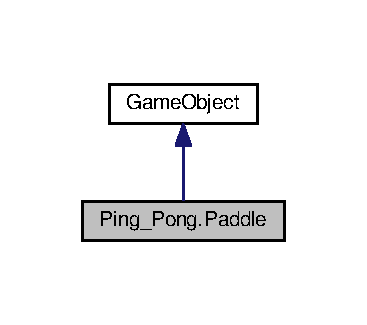
\includegraphics[width=176pt]{class_ping___pong_1_1_paddle__inherit__graph}
\end{center}
\end{figure}


Collaboration diagram for Ping\-\_\-\-Pong.\-Paddle\-:
\nopagebreak
\begin{figure}[H]
\begin{center}
\leavevmode
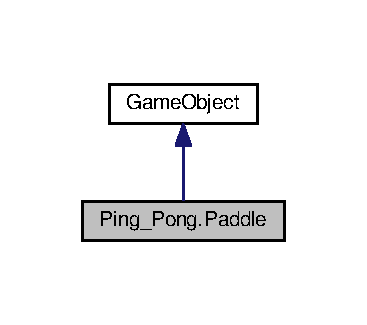
\includegraphics[width=176pt]{class_ping___pong_1_1_paddle__coll__graph}
\end{center}
\end{figure}
\subsection*{Additional Inherited Members}


\subsection{Detailed Description}


Definition at line 8 of file Paddle.\-cs.



The documentation for this class was generated from the following file\-:\begin{DoxyCompactItemize}
\item 
Pong Base/\hyperlink{_paddle_8cs}{Paddle.\-cs}\end{DoxyCompactItemize}

\hypertarget{class_ping___pong_1_1_program}{\section{Ping\-\_\-\-Pong.\-Program Class Reference}
\label{class_ping___pong_1_1_program}\index{Ping\-\_\-\-Pong.\-Program@{Ping\-\_\-\-Pong.\-Program}}
}
\subsection*{Static Private Member Functions}
\begin{DoxyCompactItemize}
\item 
static void \hyperlink{class_ping___pong_1_1_program_a9e475ac6b18638ebfc4895539e7c08ed}{Main} (string\mbox{[}$\,$\mbox{]} args)
\begin{DoxyCompactList}\small\item\em The main entry point for the application. \end{DoxyCompactList}\end{DoxyCompactItemize}


\subsection{Detailed Description}


Definition at line 5 of file Program.\-cs.



\subsection{Member Function Documentation}
\hypertarget{class_ping___pong_1_1_program_a9e475ac6b18638ebfc4895539e7c08ed}{\index{Ping\-\_\-\-Pong\-::\-Program@{Ping\-\_\-\-Pong\-::\-Program}!Main@{Main}}
\index{Main@{Main}!Ping_Pong::Program@{Ping\-\_\-\-Pong\-::\-Program}}
\subsubsection[{Main}]{\setlength{\rightskip}{0pt plus 5cm}static void Ping\-\_\-\-Pong.\-Program.\-Main (
\begin{DoxyParamCaption}
\item[{string\mbox{[}$\,$\mbox{]}}]{args}
\end{DoxyParamCaption}
)\hspace{0.3cm}{\ttfamily [inline]}, {\ttfamily [static]}, {\ttfamily [private]}}}\label{class_ping___pong_1_1_program_a9e475ac6b18638ebfc4895539e7c08ed}


The main entry point for the application. 



Definition at line 10 of file Program.\-cs.



The documentation for this class was generated from the following file\-:\begin{DoxyCompactItemize}
\item 
Pong Base/\hyperlink{_program_8cs}{Program.\-cs}\end{DoxyCompactItemize}

\chapter{File Documentation}
\hypertarget{_ball_8cs}{\section{Pong Base/\-Ball.cs File Reference}
\label{_ball_8cs}\index{Pong Base/\-Ball.\-cs@{Pong Base/\-Ball.\-cs}}
}
\subsection*{Data Structures}
\begin{DoxyCompactItemize}
\item 
class \hyperlink{class_ping___pong_1_1_ball}{Ping\-\_\-\-Pong.\-Ball}
\end{DoxyCompactItemize}
\subsection*{Namespaces}
\begin{DoxyCompactItemize}
\item 
package \hyperlink{namespace_ping___pong}{Ping\-\_\-\-Pong}
\end{DoxyCompactItemize}

\hypertarget{_game1_8cs}{\section{Pong Base/\-Game1.cs File Reference}
\label{_game1_8cs}\index{Pong Base/\-Game1.\-cs@{Pong Base/\-Game1.\-cs}}
}
\subsection*{Data Structures}
\begin{DoxyCompactItemize}
\item 
class \hyperlink{class_ping___pong_1_1_game1}{Ping\-\_\-\-Pong.\-Game1}
\begin{DoxyCompactList}\small\item\em This is the main type for your game \end{DoxyCompactList}\end{DoxyCompactItemize}
\subsection*{Namespaces}
\begin{DoxyCompactItemize}
\item 
package \hyperlink{namespace_ping___pong}{Ping\-\_\-\-Pong}
\end{DoxyCompactItemize}

\hypertarget{_game_object_8cs}{\section{Pong Base/\-Game\-Object.cs File Reference}
\label{_game_object_8cs}\index{Pong Base/\-Game\-Object.\-cs@{Pong Base/\-Game\-Object.\-cs}}
}
\subsection*{Data Structures}
\begin{DoxyCompactItemize}
\item 
class \hyperlink{class_ping___pong_1_1_game_object}{Ping\-\_\-\-Pong.\-Game\-Object}
\end{DoxyCompactItemize}
\subsection*{Namespaces}
\begin{DoxyCompactItemize}
\item 
package \hyperlink{namespace_ping___pong}{Ping\-\_\-\-Pong}
\end{DoxyCompactItemize}

\hypertarget{_debug_2_pong_01_base_8csproj_8_file_list_absolute_8txt}{\section{Pong Base/obj/x86/\-Debug/\-Pong Base.\-csproj.\-File\-List\-Absolute.\-txt File Reference}
\label{_debug_2_pong_01_base_8csproj_8_file_list_absolute_8txt}\index{Pong Base/obj/x86/\-Debug/\-Pong Base.\-csproj.\-File\-List\-Absolute.\-txt@{Pong Base/obj/x86/\-Debug/\-Pong Base.\-csproj.\-File\-List\-Absolute.\-txt}}
}

\hypertarget{_release_2_pong_01_base_8csproj_8_file_list_absolute_8txt}{\section{Pong Base/obj/x86/\-Release/\-Pong Base.\-csproj.\-File\-List\-Absolute.\-txt File Reference}
\label{_release_2_pong_01_base_8csproj_8_file_list_absolute_8txt}\index{Pong Base/obj/x86/\-Release/\-Pong Base.\-csproj.\-File\-List\-Absolute.\-txt@{Pong Base/obj/x86/\-Release/\-Pong Base.\-csproj.\-File\-List\-Absolute.\-txt}}
}

\hypertarget{_debug_2_temporary_generated_file__036_c0_b5_b-1481-4323-8_d20-8_f5_a_d_c_b23_d92_8cs}{\section{Pong Base/obj/x86/\-Debug/\-Temporary\-Generated\-File\-\_\-036\-C0\-B5\-B-\/1481-\/4323-\/8\-D20-\/8\-F5\-A\-D\-C\-B23\-D92.cs File Reference}
\label{_debug_2_temporary_generated_file__036_c0_b5_b-1481-4323-8_d20-8_f5_a_d_c_b23_d92_8cs}\index{Pong Base/obj/x86/\-Debug/\-Temporary\-Generated\-File\-\_\-036\-C0\-B5\-B-\/1481-\/4323-\/8\-D20-\/8\-F5\-A\-D\-C\-B23\-D92.\-cs@{Pong Base/obj/x86/\-Debug/\-Temporary\-Generated\-File\-\_\-036\-C0\-B5\-B-\/1481-\/4323-\/8\-D20-\/8\-F5\-A\-D\-C\-B23\-D92.\-cs}}
}

\hypertarget{_release_2_temporary_generated_file__036_c0_b5_b-1481-4323-8_d20-8_f5_a_d_c_b23_d92_8cs}{\section{Pong Base/obj/x86/\-Release/\-Temporary\-Generated\-File\-\_\-036\-C0\-B5\-B-\/1481-\/4323-\/8\-D20-\/8\-F5\-A\-D\-C\-B23\-D92.cs File Reference}
\label{_release_2_temporary_generated_file__036_c0_b5_b-1481-4323-8_d20-8_f5_a_d_c_b23_d92_8cs}\index{Pong Base/obj/x86/\-Release/\-Temporary\-Generated\-File\-\_\-036\-C0\-B5\-B-\/1481-\/4323-\/8\-D20-\/8\-F5\-A\-D\-C\-B23\-D92.\-cs@{Pong Base/obj/x86/\-Release/\-Temporary\-Generated\-File\-\_\-036\-C0\-B5\-B-\/1481-\/4323-\/8\-D20-\/8\-F5\-A\-D\-C\-B23\-D92.\-cs}}
}

\hypertarget{_debug_2_temporary_generated_file__5937a670-0e60-4077-877b-f7221da3dda1_8cs}{\section{Pong Base/obj/x86/\-Debug/\-Temporary\-Generated\-File\-\_\-5937a670-\/0e60-\/4077-\/877b-\/f7221da3dda1.cs File Reference}
\label{_debug_2_temporary_generated_file__5937a670-0e60-4077-877b-f7221da3dda1_8cs}\index{Pong Base/obj/x86/\-Debug/\-Temporary\-Generated\-File\-\_\-5937a670-\/0e60-\/4077-\/877b-\/f7221da3dda1.\-cs@{Pong Base/obj/x86/\-Debug/\-Temporary\-Generated\-File\-\_\-5937a670-\/0e60-\/4077-\/877b-\/f7221da3dda1.\-cs}}
}

\hypertarget{_release_2_temporary_generated_file__5937a670-0e60-4077-877b-f7221da3dda1_8cs}{\section{Pong Base/obj/x86/\-Release/\-Temporary\-Generated\-File\-\_\-5937a670-\/0e60-\/4077-\/877b-\/f7221da3dda1.cs File Reference}
\label{_release_2_temporary_generated_file__5937a670-0e60-4077-877b-f7221da3dda1_8cs}\index{Pong Base/obj/x86/\-Release/\-Temporary\-Generated\-File\-\_\-5937a670-\/0e60-\/4077-\/877b-\/f7221da3dda1.\-cs@{Pong Base/obj/x86/\-Release/\-Temporary\-Generated\-File\-\_\-5937a670-\/0e60-\/4077-\/877b-\/f7221da3dda1.\-cs}}
}

\hypertarget{_debug_2_temporary_generated_file___e7_a71_f73-0_f8_d-4_b9_b-_b56_e-8_e70_b10_b_c5_d3_8cs}{\section{Pong Base/obj/x86/\-Debug/\-Temporary\-Generated\-File\-\_\-\-E7\-A71\-F73-\/0\-F8\-D-\/4\-B9\-B-\/\-B56\-E-\/8\-E70\-B10\-B\-C5\-D3.cs File Reference}
\label{_debug_2_temporary_generated_file___e7_a71_f73-0_f8_d-4_b9_b-_b56_e-8_e70_b10_b_c5_d3_8cs}\index{Pong Base/obj/x86/\-Debug/\-Temporary\-Generated\-File\-\_\-\-E7\-A71\-F73-\/0\-F8\-D-\/4\-B9\-B-\/\-B56\-E-\/8\-E70\-B10\-B\-C5\-D3.\-cs@{Pong Base/obj/x86/\-Debug/\-Temporary\-Generated\-File\-\_\-\-E7\-A71\-F73-\/0\-F8\-D-\/4\-B9\-B-\/\-B56\-E-\/8\-E70\-B10\-B\-C5\-D3.\-cs}}
}

\hypertarget{_release_2_temporary_generated_file___e7_a71_f73-0_f8_d-4_b9_b-_b56_e-8_e70_b10_b_c5_d3_8cs}{\section{Pong Base/obj/x86/\-Release/\-Temporary\-Generated\-File\-\_\-\-E7\-A71\-F73-\/0\-F8\-D-\/4\-B9\-B-\/\-B56\-E-\/8\-E70\-B10\-B\-C5\-D3.cs File Reference}
\label{_release_2_temporary_generated_file___e7_a71_f73-0_f8_d-4_b9_b-_b56_e-8_e70_b10_b_c5_d3_8cs}\index{Pong Base/obj/x86/\-Release/\-Temporary\-Generated\-File\-\_\-\-E7\-A71\-F73-\/0\-F8\-D-\/4\-B9\-B-\/\-B56\-E-\/8\-E70\-B10\-B\-C5\-D3.\-cs@{Pong Base/obj/x86/\-Release/\-Temporary\-Generated\-File\-\_\-\-E7\-A71\-F73-\/0\-F8\-D-\/4\-B9\-B-\/\-B56\-E-\/8\-E70\-B10\-B\-C5\-D3.\-cs}}
}

\hypertarget{_paddle_8cs}{\section{Pong Base/\-Paddle.cs File Reference}
\label{_paddle_8cs}\index{Pong Base/\-Paddle.\-cs@{Pong Base/\-Paddle.\-cs}}
}
\subsection*{Data Structures}
\begin{DoxyCompactItemize}
\item 
class \hyperlink{class_ping___pong_1_1_paddle}{Ping\-\_\-\-Pong.\-Paddle}
\end{DoxyCompactItemize}
\subsection*{Namespaces}
\begin{DoxyCompactItemize}
\item 
package \hyperlink{namespace_ping___pong}{Ping\-\_\-\-Pong}
\end{DoxyCompactItemize}

\hypertarget{_program_8cs}{\section{Pong Base/\-Program.cs File Reference}
\label{_program_8cs}\index{Pong Base/\-Program.\-cs@{Pong Base/\-Program.\-cs}}
}
\subsection*{Data Structures}
\begin{DoxyCompactItemize}
\item 
class \hyperlink{class_ping___pong_1_1_program}{Ping\-\_\-\-Pong.\-Program}
\end{DoxyCompactItemize}
\subsection*{Namespaces}
\begin{DoxyCompactItemize}
\item 
package \hyperlink{namespace_ping___pong}{Ping\-\_\-\-Pong}
\end{DoxyCompactItemize}

\hypertarget{_assembly_info_8cs}{\section{Pong Base/\-Properties/\-Assembly\-Info.cs File Reference}
\label{_assembly_info_8cs}\index{Pong Base/\-Properties/\-Assembly\-Info.\-cs@{Pong Base/\-Properties/\-Assembly\-Info.\-cs}}
}

\hypertarget{_r_e_a_d_m_e_8md}{\section{R\-E\-A\-D\-M\-E.\-md File Reference}
\label{_r_e_a_d_m_e_8md}\index{R\-E\-A\-D\-M\-E.\-md@{R\-E\-A\-D\-M\-E.\-md}}
}

%--- End generated contents ---

% Index
\newpage
\phantomsection
\addcontentsline{toc}{chapter}{Index}
\printindex

\end{document}
